\documentclass[11pt]{article}
\usepackage{graphicx}
\usepackage[left=2.00cm, right=2.00cm, top=2.00cm, bottom=2.00cm]{geometry}
\usepackage{amsmath}
\usepackage[colorlinks]{hyperref}
\usepackage[backend=biber]{biblatex}
\usepackage{eurosym}
\usepackage[dvipsnames]{xcolor} 
\usepackage{subcaption}
\usepackage{accents}
\usepackage[capitalise]{cleveref}

\addbibresource{main.bib}
\graphicspath{{figures/}}

\crefname{relation}{Rel.}{Rels.}
\creflabelformat{relation}{(#2#1#3)}
\crefname{constraint}{Constr.}{Constrs.}
\creflabelformat{constraint}{(#2#1#3)}

\setlength\parindent{8pt}

\newcommand{\ie}{\textit{i.e.} }
\newcommand{\eg}{\textit{e.g.} }

\newcommand{\ubar}[1]{\underaccent{\bar}{#1}}
\newcommand{\note}[1]{\textcolor{Orange}{#1}}
\newcommand{\vpad}{\vspace{1mm}}

\newcommand{\generation}[1][n]{g_{#1,s,t}}
\newcommand{\generationpotential}{\bar{g}_{n,s,t}}
\newcommand{\generationshare}[1][n]{\omega_{#1,s,t}}
\newcommand{\generationnodal}[1][n]{g_{#1,t}}
\newcommand{\capacityGeneration}{G_{n,s}}
\newcommand{\capacityFlow}{F_{\ell}}
\newcommand{\capexGeneration}{c_{n,s}}
\newcommand{\capexFlow}{c_{\ell}}
\newcommand{\opexGeneration}[1][n]{o_{#1,s}}
\newcommand{\demand}[1][n]{d_{#1,a,t}}
\newcommand{\demandnodal}[1][n]{d_{#1,t}}
\newcommand{\demandshare}[1][n]{\omega_{#1,a,t}}
\newcommand{\utility}{U_{n,a,t}}
\newcommand{\incidence}[1][n]{K_{#1,\ell}}
\newcommand{\ptdf}[1][n]{H_{\ell,#1}}
\newcommand{\ptdfEqual}[1][n]{\ptdf[#1]^\circ}
\newcommand{\slackflow}{k_{\ell}}
\newcommand{\slack}[1][n]{k_{#1}}
\newcommand{\Slack}{k_{m,n}}
\newcommand{\mulowergeneration}[1][n]{\ubar{\mu}_{#1,s,t}}
\newcommand{\muuppergeneration}[1][n]{\bar{\mu}_{#1,s,t}}
\newcommand{\mulowerflow}{\ubar{\mu}_{\ell,t}}
\newcommand{\muupperflow}{\bar{\mu}_{\ell,t}}
\newcommand{\lmp}[1][n]{\lambda_{#1,t}}
\newcommand{\flow}{f_{\ell,t}}
\newcommand{\cycle}{C_{\ell,c}}
\newcommand{\impedance}{x_\ell}
\newcommand{\cycleprice}{\lambda_{c,t}}
\newcommand{\injection}{p_{n,t}}
\newcommand{\netconsumption}[1][n]{p^{-}_{#1,t}}
\newcommand{\netproduction}[1][n]{p^{+}_{#1,t}}
\newcommand{\selfconsumption}[1][n]{p^{\circ}_{#1,t}}

\newcommand{\totalnetconsumption}{p^{-}_{t}}
\newcommand{\totalnetproduction}{p^{+}_{t}}
\newcommand{\totalselfconsumption}{p^{\circ}_{t}}

\newcommand{\lagrangian}{\mathcal{L}}

\newcommand{\allocatePeer}[1][m \rightarrow n]{A_{#1,t}}
\newcommand{\allocateFlow}[1][n]{F_{#1,\ell,t}}
\newcommand{\allocateTransaction}[1][m \rightarrow n]{A_{#1,\ell,t}}
\newcommand{\allocateCapexGeneration}[1][n]{\mathcal{C}^{G}_{#1,t}}
\newcommand{\allocateCapexFlow}[1][n]{\mathcal{C}^{F}_{#1,t}}
\newcommand{\allocateOpex}[1][n]{\mathcal{O}_{#1,t}}
\newcommand{\allocateEmissionCost}[1][n]{\mathcal{E}_{#1,t}}

\newcommand{\emission}[1][n]{e_{#1,s}}
\newcommand{\emissionPrice}{\mu_{\text{CO2}}}
\newcommand{\megawatthour}{MWh$_\text{el}$}
\newcommand{\totalcost}{\mathcal{TC}}
\newcommand{\impactcapexgeneration}{\Phi_{n,s,t}}
\newcommand{\impactcapexflow}{\Phi_{\ell,t}}

%math 
\newcommand{\resultsin}[1]{\hspace{12pt} \bot  \hspace{12pt} #1}
\newcommand{\Forall}[1]{\hspace{20pt} \forall \,\, #1 }
\newcommand{\pdv}[2]{\frac{\partial #1}{\partial #2}}

\begin{document}


\title{From Linear Optimization to Transmission Cost Allocation}
\author{Fabian Hofmann}

\maketitle

% \begin{abstract}
% The abstract text goes here.
% \end{abstract}

In the following, we show how Flow Allocation (FA) can be used for decomposing Locational Marginal Prices (LMP) in a linear optimized power system. We begin by revising the fundamentals of the Power Transfer Distribition Factors (PTDF) and the role of the slack, which plays a key role for FA. This will lead us to a generalized form of peer-to-peer allocations and transmission usage allocations based on the choice of slack. In a second step, we breakdown the full Lagrangian of a cost-optimization for a network with transmission and generation capacity expansion. By taking into account sensitivities of the flow with respect to changes in the nodal generation, we are able to derive a cost allocation which directly links to FA.  

\subsubsection*{Nomenclature}

\begin{table}[h]
	\centering
	\begin{tabular}{ll}
        $\demand$ & Electric demand per bus $n$, demand type $a$, time step $t$ in MW  \vpad \\
        $\generation$ & Electric generation per bus $n$, carrier $s$, time step $t$  in MW \vpad \\
        $\flow$ & Active power flow on line $\ell$, time step $t$ in MW   \vpad \\
        $\opexGeneration$ & Operational cost (OPEX) in \euro/MW \vpad \\
        $\capexGeneration$ & Capital Expenditure (CAPEX) in \euro/MW \vpad \\
        $\capexFlow$  & CAPEX per transmission line $\ell$ in \euro/MW  \vpad \\
        $\capacityGeneration$ & Generation capacity in MW \vpad \\
        $\capacityFlow$ & Transmission capacity in MW \vpad \\
        $\incidence$ & Incidence matrix \vpad \\
        $\injection$ & Net nodal injection in MW, \ie $\left( \generationnodal - \demandnodal \right)$  \vpad \\
        $\netproduction$ & Net nodal production in MW, \ie $\text{min}\left( \injection, 0 \right)$ \vpad \\
        $\netconsumption$ & Net nodal consumption in MW, \ie $\text{min}\left( - \injection, 0 \right)$ \vpad \\ 
        $\selfconsumption$ & Nodal self-consumption in MW, \ie $\text{min}\left( \netproduction, \netconsumption \right)$
	\end{tabular}
\end{table}




\subsubsection*{Power Transfer Distribition Factors}


The Power Transfer Distribition Factors (PTDF) $\ptdf$ determine the changes in the flow on line $\ell$ for one unit (typically one MW) of net power production at bus $n$. Thus with a fix demand $\demand$, they directly link the generation $\generation$ to the flow on each line according to
\begin{align}
 \flow\left( \generation\right)  = \sum_n \ptdf \left( \sum_s \generation- \sum_a \demand \right)  
 \label{eq:flow_from_ptdf}
\end{align}
The PTDF have a degree of freedom: The slack $\slack$ denotes the contribution of bus $n$ to balancing out total power excess or deficit in the system. It can be dedicated to one bus, a sinlge ``slackbus``, or to several or all buses. The choice of slack modifies the PTDF accordingly 
\begin{align}
 \ptdf = \ptdfEqual - \sum_m \ptdfEqual[m]  \, \slack[m]
 \label{eq:ptdf_slacked}
\end{align}
where $\ptdfEqual$ denote the PTDF with equally distributed slack.
When bus $n$ injects excess power, it has to flow to the slack; when bus $n$ extract deficit power, it has to come from the slack. Summing over all ingoing and outgoing flow changes resulting from an positive injection at $n$ yields again the slack 
\begin{align}
\sum_\ell \incidence[m] \, \ptdf =  \delta_{m,n} - \slack[m] 
\label{eq:slack}
\end{align}
where $\delta_{m,n}$ on the right hand side represents the positive injection at $n$.

\subsubsection*{Flow Allocation} \label{sec:flow_allocation}

As shown above, the choice of slack $\slack[m]$ decides on the generators and lines to which power imbalances are distributed to. Established flow allocation schemes haved used this relation and define the slack $\slack[m]$ in order to allocate power flows and exchanges. According to the Equivalent Bilateral Exchanges (EBE) for example, the net demand of bus $n$ is covered by all other buses proportional to their net power production. The Marginal Participation (MP) on the other hand allows to allocate power also to buses with net demand and net production at the same time. In the following we focus on the power that is allocated to net consumers in the network. \\  

For a generic slack, the effective power which is produced at bus $m$ and assigned to consumers at bus $n$ is given by
\begin{align}
%  \allocatePeer = \demandnodal \, \slack[m]   \Forall{n,t}
 \allocatePeer = \selfconsumption + \netconsumption \, \slack[m]   \Forall{n,t}
 \label{eq:allocate_peer}
\end{align}
which we will refer to as the peer-to-peer allocation. It consists of two terms. The first term is the power which is produced at bus $n$ and at the same time consumed at bus $n$, namely the self-consumption $\selfconsumption$. We set this quantity to the minimum of nodal generation and demand, \ie $\selfconsumption = \text{min}(\generation, \demand)$, that is as long as the nodal generation does not exceed the nodal demand, it cannot be exported and assigned to other buses. The second term reflects the net deficit power of bus $n$ which is provided by the slack $\slack$. Following this concept, $\allocatePeer$ splits the electricity demand $\demandnodal$ to different providing buses. 

Multipying the PTDF with the net demand $\netconsumption$ results in the flow induced by all imports to $n$
\begin{align}
%  \sum_m \allocateTransaction = - \demandnodal  \, \ptdf \Forall{n,\ell,t}
 \sum_m \allocateTransaction = - \netconsumption  \, \ptdf \Forall{n,\ell,t}
 \label{eq:allocate_transaction}
\end{align}
where the PTDF include the slack $\slack[m]$ according to \cref{eq:ptdf_slacked}. The slack $\slack[m]$ in \cref{eq:allocate_peer,eq:allocate_transaction} should be chosen such that the sum over all recipients $n$ in $\allocatePeer$ results in the nodal production, thus
\begin{align}
 \sum_n \allocatePeer = \generationnodal[m] \Forall{m,s,t}
 \label{eq:generator_sum}
\end{align}
where $\generationnodal = \sum_s \generation$ is the nodal generation.
Then, weighted by the nodal production share $\generationshare[m] = \generation[m]/\generationnodal[m]$ the allocation distributes all power pruduced by generator $(m,s)$,
\begin{align}
  \sum_n \generationshare[m] \, \allocatePeer = \generation[m] \Forall{m,s,t}
  \label{eq:recipients_sum}
\end{align}
and the sum over all producers $m$ and recipients $n$ in $\allocateTransaction$ results in the power flow on line $\ell$,
\begin{align}
 \sum_{m,n} \allocateTransaction = \flow \Forall{\ell,t}
 \label{eq:transaction_sum}
\end{align}
\\


\subsubsection*{Network Optimisation}

% Maximise $f(x_l)$, with equality constraints $g_i(x_l)$ and inequality constraints $h_j(x_l)$
% 
% \begin{align}
%  \mathcal {L}(x_l,\lambda_i, \mu_j)=f(x_l)-\sum_i \lambda_i \, g_i(x_l) - \sum_j \mu_j \, h_j(x_l)
% \end{align}
% ...
% 

We linearly cost-optimize the capacity and dispatch of a simple power system. 

\begin{align}
    \underset{\demand, \generation, \capacityGeneration}{\text{max}}
    \left(\sum_{n,s} \capexGeneration \capacityGeneration - \sum_{n, s, t} \opexGeneration \generation - \sum_{\ell} \capexFlow \, \capacityFlow \right) \label{eq:minisation}
\end{align}
% where 
% \begin{itemize}
% \item[] $\utility$ denotes the utility function per bus $n$, demand type $a$ time step $t$ 
%  \item[] $\demand$ denotes the eletric demand 
%  \item[] $\capexGeneration$ denotes the capital expenditure (CAPEX) per node $n$ and generator type $s$
%  \item[] $\capacityGeneration$ denotes the generation capacity
%  \item[] $\opexGeneration$ denotes the operational cost (OPEX)
%  \item[] $\generation$ denotes the net generation in MW
%  \item[] $\flow$ denotes the active power flow on line $\ell$
%  \item[] $\capexFlow$ denotes the CAPEX per transmission line 
%  \item[] $\capacityFlow$ denotes the transmission capacity.
subject to following physical constraints. 
\\
% In the following we neglect the utility $\utility$ of the nodal demand while fixing the demand $\demand$ to a predefined time-series. \\


The nodal balance constraint ensures that the amount of power that flows into a bus equals the power that flows out of a bus, thus reflects the Kirchhoff Current Law (KCL)
\begin{align}
    \sum_l \incidence \, \flow - \sum_s \generation + \sum_a \demand &= 0 \resultsin{\lmp} \Forall{n,t}
    \label[constraint]{eq:nodal_balance_lin}
\end{align}
Its shadow price mirrors the Locational Marginal Prizes (LMP) $\lmp$ per bus and time step. In a power market this is the \euro/\megawatthour-price which a consumer has to pay. Note that the flow $\flow$ in \cref{eq:nodal_balance_lin} is a passive variable only, given by \cref{eq:flow_from_ptdf}.\\

The generation $\generation$ is constraint to its nominal capacity
\begin{align}
 \generation - \generationpotential \capacityGeneration  &\le 0 \resultsin{\muuppergeneration} \Forall{n,s,t} 
 \label[constraint]{eq:upper_generation_capacity_constraint}\\ 
 - \generation &\le 0 \resultsin{\mulowergeneration} \Forall{n,s,t} 
 \label[constraint]{eq:lower_generation_capacity_constraint}
 \end{align}
where $\generationpotential \in \left[ 0,1\right]$ is the capacity factor for renewable generators. The constraints yield the KKT variables $\muuppergeneration$ and $\mulowergeneration$ which due to complementary slackness,
\begin{align}
\muuppergeneration \left( \generation - \generationpotential \, \capacityGeneration \right)  &= 0  \Forall{n,s,t} 
\label{eq:complementary_slackness_upper_generation} \\
\mulowergeneration  \, \generation &= 0 \Forall{n,s,t}
\label{eq:complementary_slackness_lower_generation} 
\end{align}
are only non-zero if the corresponding constraint is binding. \\


The transmission capacity $\capacityFlow$ limits the flow $\flow$ in both directions, such that 
\begin{align}
 \flow - \capacityFlow &\le 0 \resultsin{\muupperflow} \Forall{\ell,t} 
 \label[constraint]{eq:upper_flow_capacity_constraint} \\
 - \flow - \capacityFlow &\le 0 \resultsin{\mulowerflow} \Forall{\ell,t} 
 \label[constraint]{eq:lower_flow_capacity_constraint}
\end{align}
The yielding KKT variables $\muupperflow$ and $\mulowerflow$ are only non-zero if $\flow$ is limited by the trasmission capacity in positive or negative direction, i.e. \cref{eq:upper_flow_capacity_constraint} or \cref{eq:lower_flow_capacity_constraint} are binding. The complementary slackness 
\begin{align}
 \muupperflow \left( \flow - \capacityFlow \right)  &= 0 \Forall{\ell,t}
 \label{eq:complementary_slackness_upper_flow} \\
 \mulowerflow \left( \flow - \capacityFlow \right) &=  0 \Forall{\ell,t}
 \label{eq:complementary_slackness_lower_flow} 
\end{align}
set the respective KKT for flows staying below the thermal limit to zero. 
\\



\subsubsection*{Decomposing the Locational Marginal Prices and Allocating the Electricity Costs}
\begin{align}
 \lagrangian\left(\generation, \capacityGeneration, \capacityFlow, \boldsymbol{\lambda}, \boldsymbol{\mu} \right)   = &- \sum_{n,s} \capexGeneration \capacityGeneration - \sum_{n, s, t} \opexGeneration \generation - \sum_{\ell} \capexFlow \, \capacityFlow  \\
 &- \sum_{n,t} \lmp \left(\sum_\ell \incidence \, \flow  - \sum_s \generation + \sum_a \demand  \right)  \\ 
%  &- \sum_{\ell,c,t} \cycleprice \, \cycle \, \impedance \, \flow  \label[constraint]{eq:langrange_cycle_constraint} \\ 
 &- \sum_{n,s,t} \muuppergeneration \left( \generation - \generationpotential \capacityGeneration \right)  + \sum_{n,s,t} \mulowergeneration \generation  \\
 &- \sum_{\ell,t} \muupperflow \left( \flow - \capacityFlow \right) + \sum_{\ell,t} \mulowerflow \left( \flow + \capacityFlow \right)     
\end{align}
% 
where $\boldsymbol{\lambda} = \left\lbrace \lmp \right\rbrace $ and $\boldsymbol{\mu} = \left\lbrace \muuppergeneration, \mulowergeneration, \muupperflow, \mulowerflow \right\rbrace $ denote the set of related KKT variables. The global maximum of the Lagrangian requires stationarity with respect to all variables. The stationarity of the generation capacity variable leads to 
\begin{align}
 \pdv{\lagrangian}{\capacityGeneration}  = 0 \hspace{10pt} \rightarrow \hspace{10pt} \capexGeneration =  \sum_t \muuppergeneration \, \generationpotential  \Forall{n,s}
 \label{eq:capexGeneration_duality}
\end{align}

the stationarity of the transmission capacity to
\begin{align}
 \pdv{\lagrangian}{\capacityFlow} = 0 \hspace{10pt} \rightarrow \hspace{10pt} \capexFlow =  \sum_t \left( \muupperflow - \mulowerflow \right) \Forall{\ell}
 \label{eq:capexFlow_duality}
\end{align}


and the stationarity of the generation to 
\begin{align}
 \pdv{\lagrangian}{\generation} &= 0  &\Forall{n,s} \\
 \rightarrow \hspace{10pt}  \opexGeneration &=  \lmp - \muuppergeneration + \mulowergeneration - \sum_{\ell} \left( \muupperflow - \mulowerflow\right)  \, \ptdf - \sum_{m,\ell}\lmp[m] \, \incidence[m] \, \ptdf   &\Forall{n,s} \label{eq:opex_duality}
\end{align}
% 
For the latter, we used \cref{eq:flow_from_ptdf} which sets the derivative of the flow with respect to the generation to 
\begin{align}
\pdv{\flow}{\generation} = \ptdf                                                                                                                                                   \end{align}
\Cref{eq:capexGeneration_duality,eq:capexFlow_duality,eq:opex_duality} show how the capital and operational prices translate into dual variables. \\

Note that \cref{eq:opex_duality} must hold for every choice of slack in the PTDF. According to \cref{eq:ptdf_slacked,eq:slack}, setting the slack to $\slack = \delta_{m,n}$ results in $\ptdf = \sum_\ell \incidence[m] \, \ptdf = 0$. This leads to our first represantion for Locational Market Price, which we will refer to as the ``Island Solution``,
\begin{align}
\lmp  =  \opexGeneration + \muuppergeneration - \mulowergeneration \Forall{n,s,t}
\label{eq:lmp1}
\end{align}
Accordingly, the LMP is directly determined by the local operational price and prices for the generation capacity constraint. 
However, from the Island Solution, we can derive a second representation for the LMP. Feeding \cref{eq:lmp1} back into \cref{eq:opex_duality} and applying \cref{eq:slack}, finally leads to 
\begin{align}
\lmp =  - \sum_\ell \left( \muupperflow - \mulowerflow\right) \ptdf + \sum_m \left( \opexGeneration[m] + \muuppergeneration[m] - \mulowergeneration[m] \right) \slack[m] \Forall{n,s,t} 
\label{eq:lmp2}
\end{align}
This equation generalizes the former Island Solution for the LMP which again can be reproduced by setting $\slack[m] = \delta_{m,n}$. It depicts the interdependence of the LMP, that is how $\lmp$ can be decomposed to operational prices and prices for capacity constraints from all generators and transmission lines in the system. 
% As shown above, the choice of slack $\slack[m]$ in \cref{eq:lmp2} decides on the generators and lines to which the nodal price at $n$ is allocated to. 
Further, \cref{eq:lmp2} reveals a crucial connection of the nodal electricity cost to the above presented flow allocation:
Multiplying both sides of \cref{eq:lmp2}  with the net nodal demand $\netconsumption$
breaks down the costs of power import to $n$. Then adding the price of the selfconsumption $\lmp \selfconsumption$ to both sides, finally breaks down the total gross demand cost at $n$,

\begin{align}
 \lmp \, \demandnodal = \allocateCapexFlow + \allocateOpex + \allocateCapexGeneration \Forall{n,t}
 \label{eq:lmp_allocation}
\end{align}

with the allocated payments: \\
\begin{align}
 \allocateOpex &= 
 \sum_{m,s} \allocateOpex[n \rightarrow (m,s)]= 
 \sum_{m,s} \opexGeneration[m] \, \generationshare[m] \, \allocatePeer 
 &\text{OPEX for generators} 
\label{eq:allocate_opexGeneration}\\
 \allocateCapexGeneration &= 
 \sum_{m,s} \allocateCapexGeneration[n \rightarrow (m,s)] = 
 \sum_m \muuppergeneration[m] \, \generationshare[m] \, \allocatePeer
 &\text{CAPEX for the generators} 
\label{eq:allocate_capexGeneration} \\
 \allocateCapexFlow &=  
 \sum_{\ell} \allocateCapexFlow[n \rightarrow \ell] =  
 \sum_{m,\ell} \left( \muupperflow - \mulowerflow\right) \allocateTransaction  
 &\text{CAPEX for the transmission system} 
\label{eq:allocate_capexFlow}
\end{align}
Note that we used \cref{eq:allocate_peer,eq:allocate_transaction} which determine the peer-to-peer transactions between $m \rightarrow n$ and the corresponding usage of lines. \Cref{eq:lmp_allocation,eq:allocate_opexGeneration,eq:allocate_capexGeneration,eq:allocate_capexFlow} show how physically allocated flows on the basis of the slack directly tranlate into a cost allocation.\\ 

Let's have a look at the allocated OPEX first. Consumers at bus $n$ retrieve power from different generators $(m,s)$ and accordingly compensate their operational costs. The OPEX allocation behaves like P2P tradings between producers and consumers with fixed production prices. In this way, the generator $(m,s)$ retrieves the exact amount of money from consumers that it spends on the operation. In other words, all OPEX payments to generator (m,s) sum up to the total OPEX spent at (m,s), thus 
\begin{align}
\sum_{n} \allocateOpex[n \rightarrow (m,s)] = \opexGeneration \, \generation
\label{eq:no_profit_opex}
\end{align}


The CAPEX allocation for generators reveil a similar relation. According to the polluter pays principle, it differentiates between consumers who are `responsible` for investments and those who are not. If $\muuppergeneration > 0$, the upper Capacity \cref{eq:upper_generation_capacity_constraint} is binding. Thus it is these times steps which push investments in $\capacityGeneration$. If $\muuppergeneration = 0$, the generation $\generation$ is not bound and investments are not necessary. 
When summing over all CAPEX payments to generator $(m,s)$ each generator retrieves exactly the cost that were spent to build the capacity $\capacityGeneration$,

\begin{align}
 \sum_{n,t} \allocateCapexGeneration[n \rightarrow (m,s)] = \capexGeneration \, \capacityGeneration
\label{eq:no_profit_capex_generation}
\end{align}
where we used \cref{eq:complementary_slackness_upper_generation,eq:capexGeneration_duality}. So in total, throughout all time steps each generator $(m,s)$ receives the money it spends for invesments and operation (non-profit rule). 
% The non-profit rule can also be seen when looking at the the total revenue per generator, 
% \begin{align}
%  \sum_t \lmp \, \generation &= \sum_t \opexGeneration \generation + \muuppergeneration \generation - \mulowergeneration \, \generation &\Forall{n,s} \\
%  &= \sum_t \opexGeneration \, \generation + \capexGeneration \, \capacityGeneration &\Forall{n,s}
% \end{align}
%  where we multiplied both sides of \cref{eq:lmp1} by the generation and using the complementary slackness.  
\\ 

The allocation of CAPEX for the transmission system $\allocateCapexFlow$ builds up on the KKT variables $\muupperflow$ and $\mulowerflow$. Again the latter translate to the necessity of transmission invesments at $\ell$ at time $t$. Consumers which retrieve power flowing on congested lines, yielding a bound \cref{eq:upper_flow_capacity_constraint} or \eqref{eq:lower_flow_capacity_constraint}, pay compensations for the resulting investments. Again the sum of all CAPEX payments to line $\ell$ equal the total CAPEX spent, thus

\begin{align}
 \sum_{n,t} \allocateCapexFlow[n \rightarrow \ell] = \capexFlow \, \capacityFlow  
\end{align}
where we used the complementary slackness \cref{eq:complementary_slackness_upper_flow,eq:complementary_slackness_lower_flow} and the fact that summing over all sources $m$ and sinks $n$ the allocation equals the actual power flow as stated in \cref{eq:transaction_sum}. 
% A similar relation applies for the transmission CAPEX. Mulplying both side of \cref{eq:opex_duality} by the nodal injection $\sum_s \generation - \sum_a \demand$ and using the complementary slackness ...
% shows that the CAPEX per line amounts to the total congestion revenue
% \begin{align}
% \capexFlow \, \capacityFlow &= - \sum_{n,t} \lmp \, \incidence \, \flow \Forall{\ell} \label{eq:non_profit_branch}
% \end{align}
% The transmission lines carry power from nodes with lower LMP to nodes with higher LMP, the price difference times the transported power is their congestion revenue. \note{Sign is different to Tom's paper (there a minus is missing).}


\subsubsection*{Adding CO$_2$ Constraints}

Imposing an additional CO$_2$ constraint limiting the total emission to K,  
\begin{align}
 \sum_{n,s,t} \emission \, \generation \le \text{K} \resultsin{\emissionPrice} 
 \label[constraint]{eq:co2_constraint}
\end{align}
with $\emission$ being the emission factor in tonne-CO$_2$ per \megawatthour, returns an effective CO$_2$ price $\emissionPrice$ in \euro/tonne-CO$_2$. 
% The CO$_2$ price shifts the right hand side of the non-profit relation for generators \cref{eq:non_profit_generator} to
% 
% \begin{align}
% \capexGeneration \, \capacityGeneration + \sum_{t} \opexGeneration \, \generation &= \sum_{t} \left( \lmp - \emission \, \emissionPrice \right)  \, \generation \Forall{n,s} 
% \label{eq:non_profit_generator_emission}
% \end{align}
% This shows nicely the duality for exchanging the CO$_2$ \cref{eq:co2_constraint} for a shifted OPEX which includes the CO$_2$ costs
As shown in ... the constraint can be translated in a dual price which shift the operational price per generator
\begin{align}
\opexGeneration \rightarrow \opexGeneration + \emission \, \emissionPrice \label[relation]{eq:shift_opex_by_emission_cost}
\end{align}
This leads to allocated CO$_2$ cost compensation of node $n$ of
 \begin{align}
 \allocateEmissionCost &= \emissionPrice \, \sum_{m,s} \emission[m] \, \generationshare[m] \, \allocatePeer \Forall{n,t} \label{eq:allocate_emissionPrice}
\end{align}
which expands the allocation of the electricity cost in \cref{eq:lmp_allocation} to 
\begin{align}
 \lmp \, \demandnodal = \allocateCapexFlow + \allocateOpex + \allocateCapexGeneration  + \allocateEmissionCost \Forall{n,t}
 \label{eq:lmp_allocation_with_emission}
\end{align}


\newpage
\section*{Showcase}

\subsection*{Network with CO$_2$ constraint}
We illustrate the flow based cost allocation under use of the fictive network shown in \cref{fig:network}. It consists of nine buses and ten time steps. The solver optimizes the capacity of two generators, wind and gas, per bus. ...   

\begin{figure}[h]
    \centering
    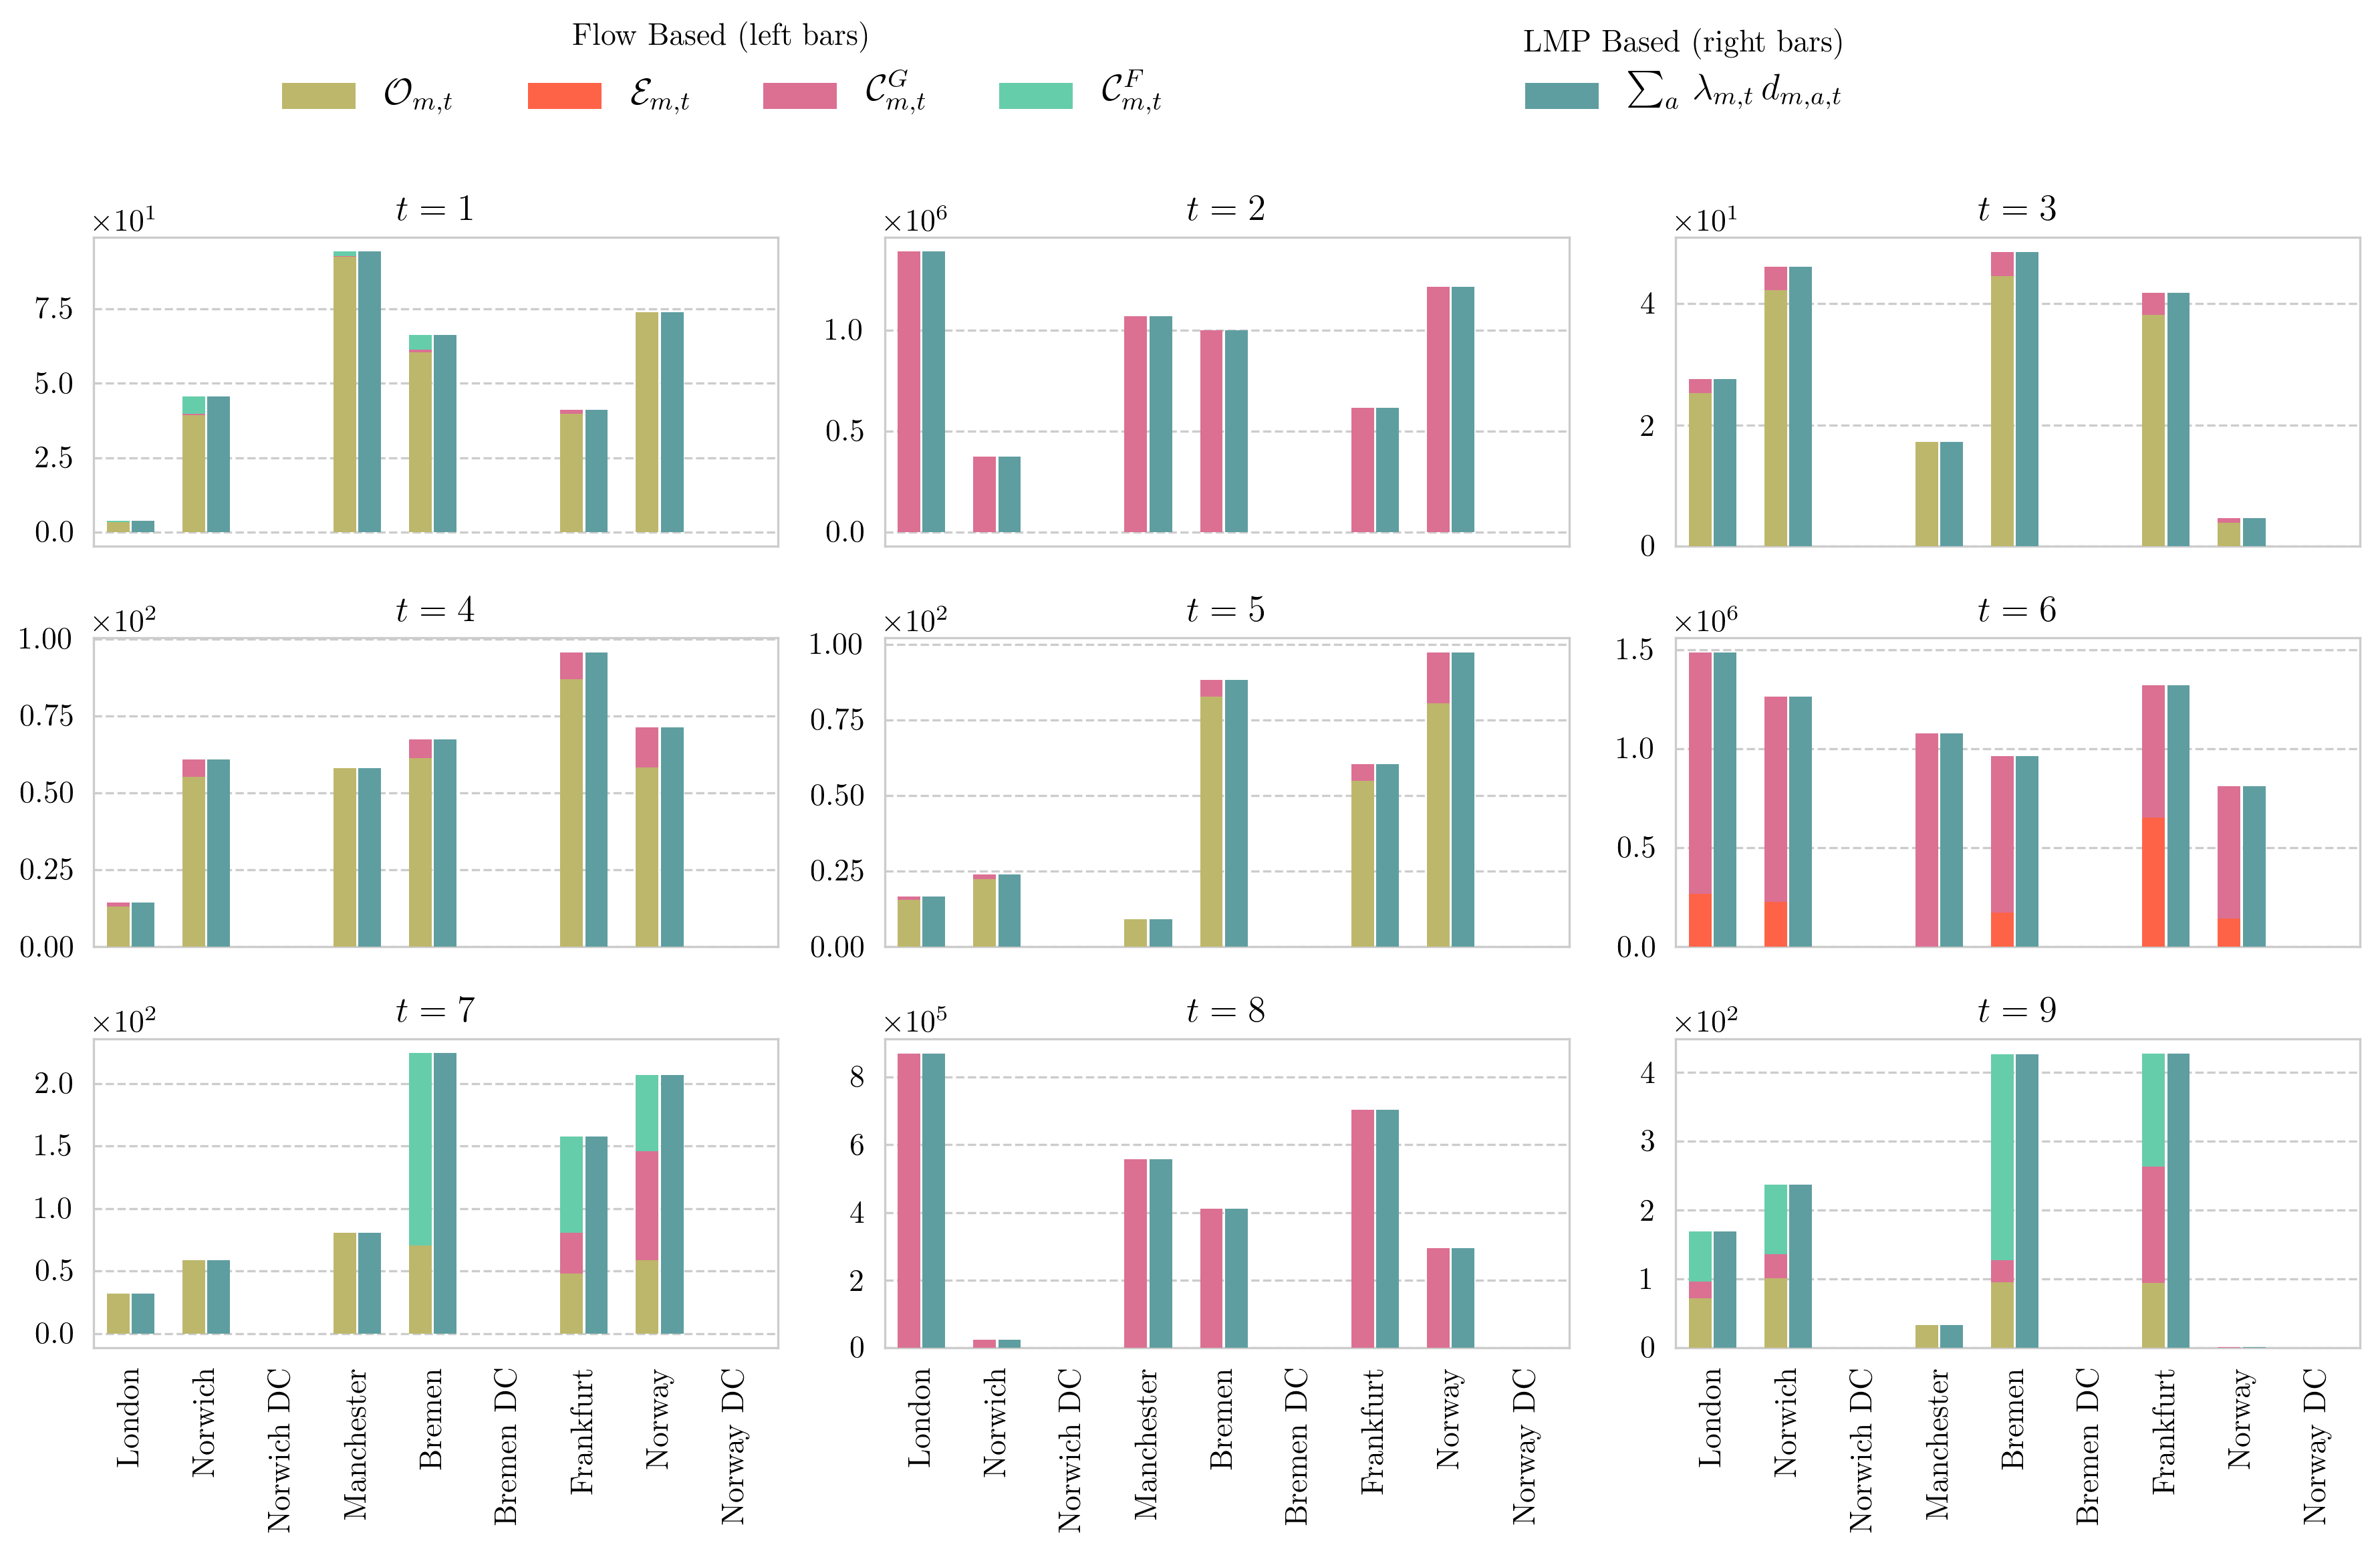
\includegraphics[width=\textwidth]{compare_allocation.png}
    \caption{Comparison between the flow based cost allocation and the LMP based cost per consumer. The left bars consist of the allocated OPEX $\allocateOpex$, the allocated CO$_2$ cost $\allocateEmissionCost$, the allocated generator CAPEX $\allocateCapexGeneration$ and transmission CAPEX $\allocateCapexFlow$, while the right bars show the of the nodal consumption times the LMP. }
    \label{fig:cost_allocation}
\end{figure}

\begin{figure}[h]
\begin{subfigure}{.5\textwidth}
\centering
 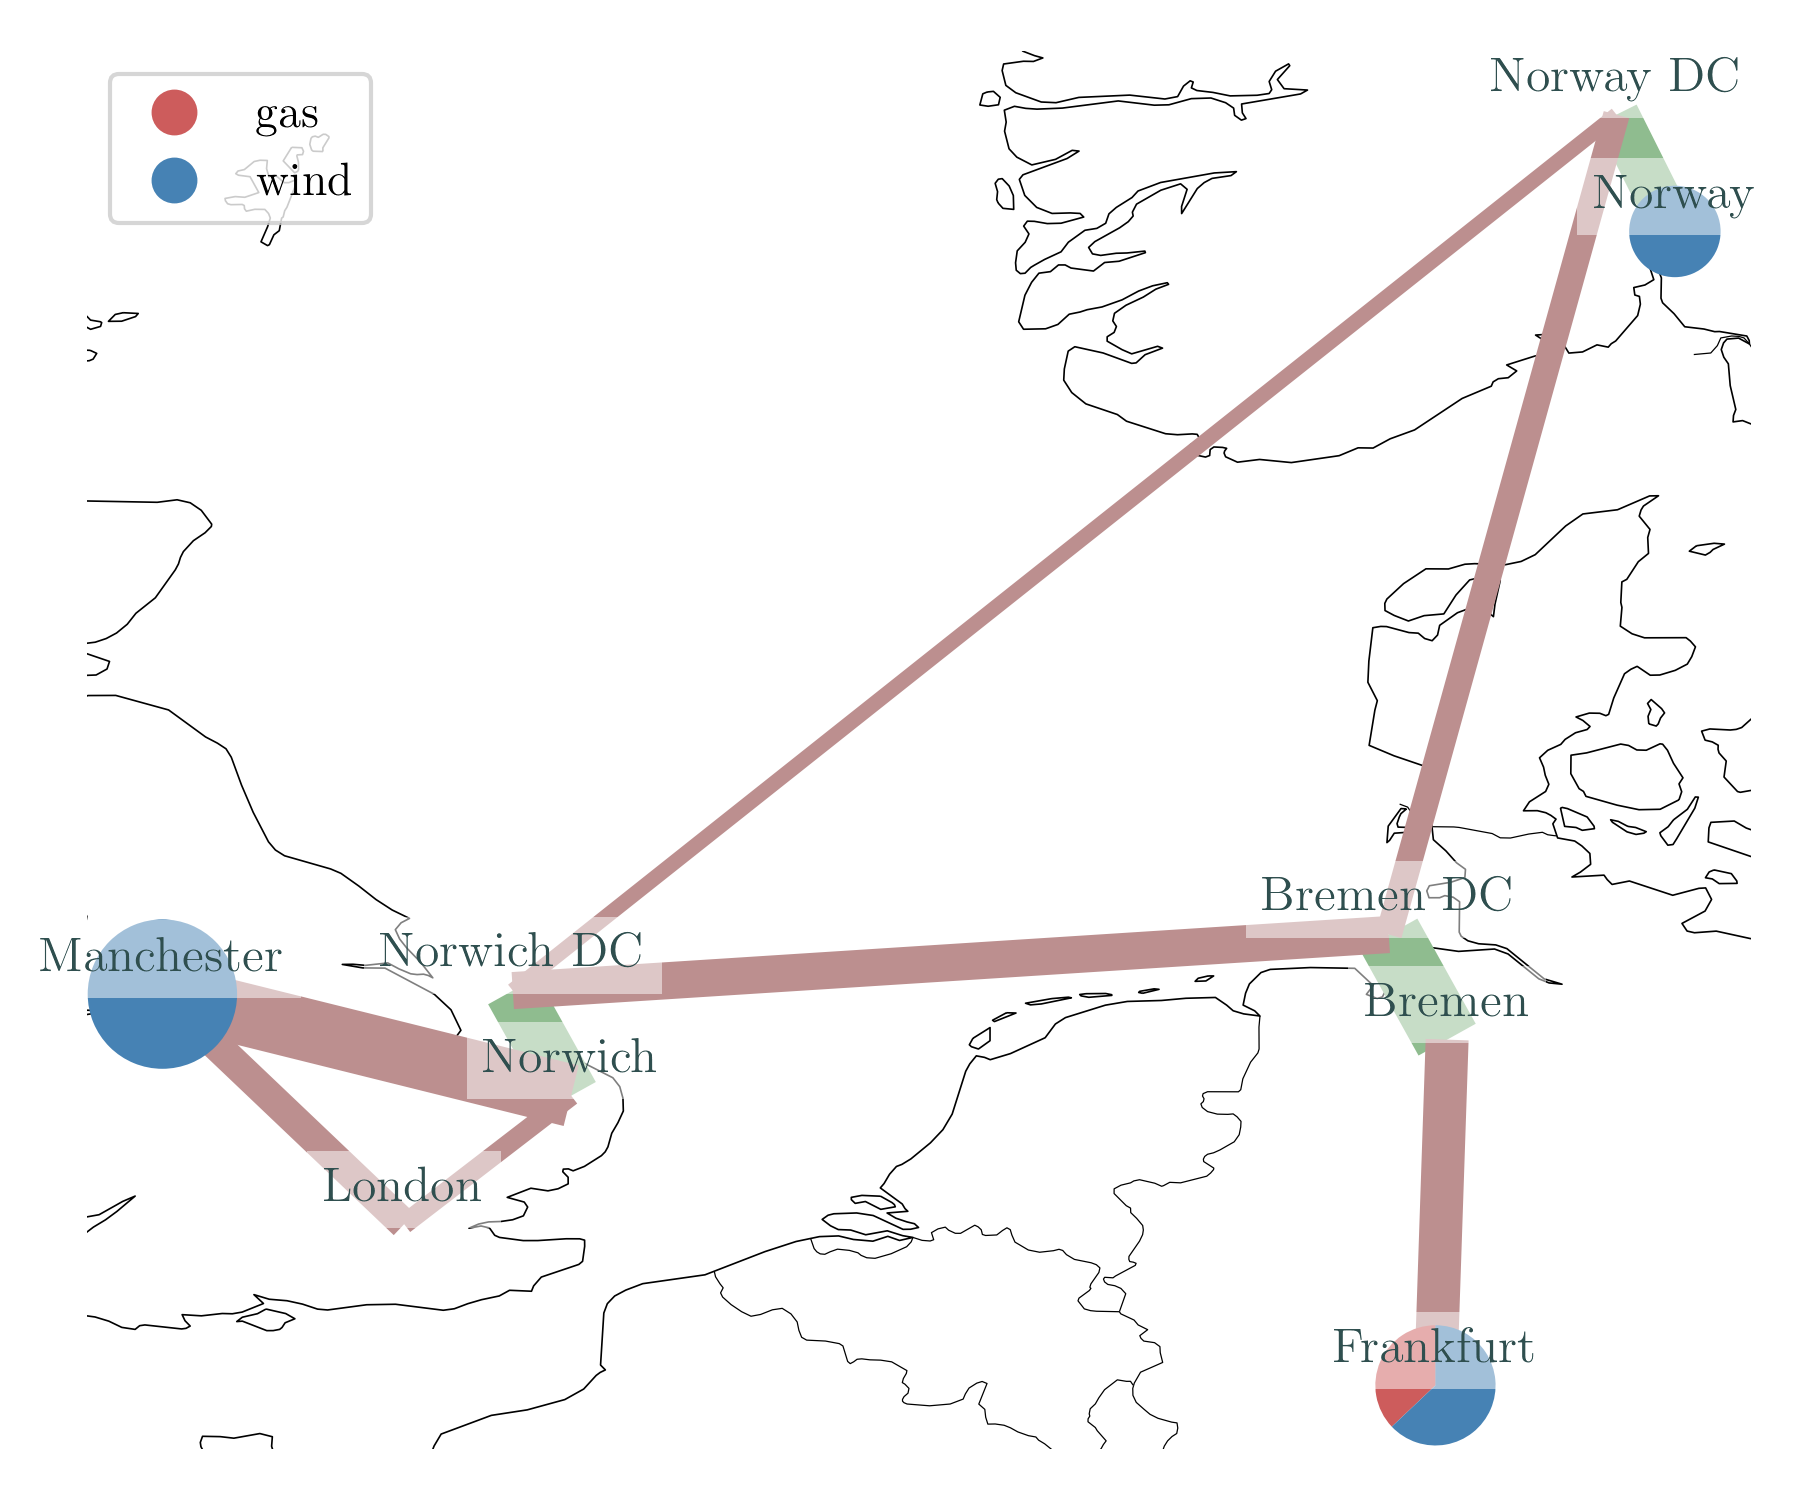
\includegraphics[width=\textwidth]{network.png}
 \caption{}
 \label{fig:network}
\end{subfigure}
\begin{subfigure}{.5\textwidth}   
    \centering
    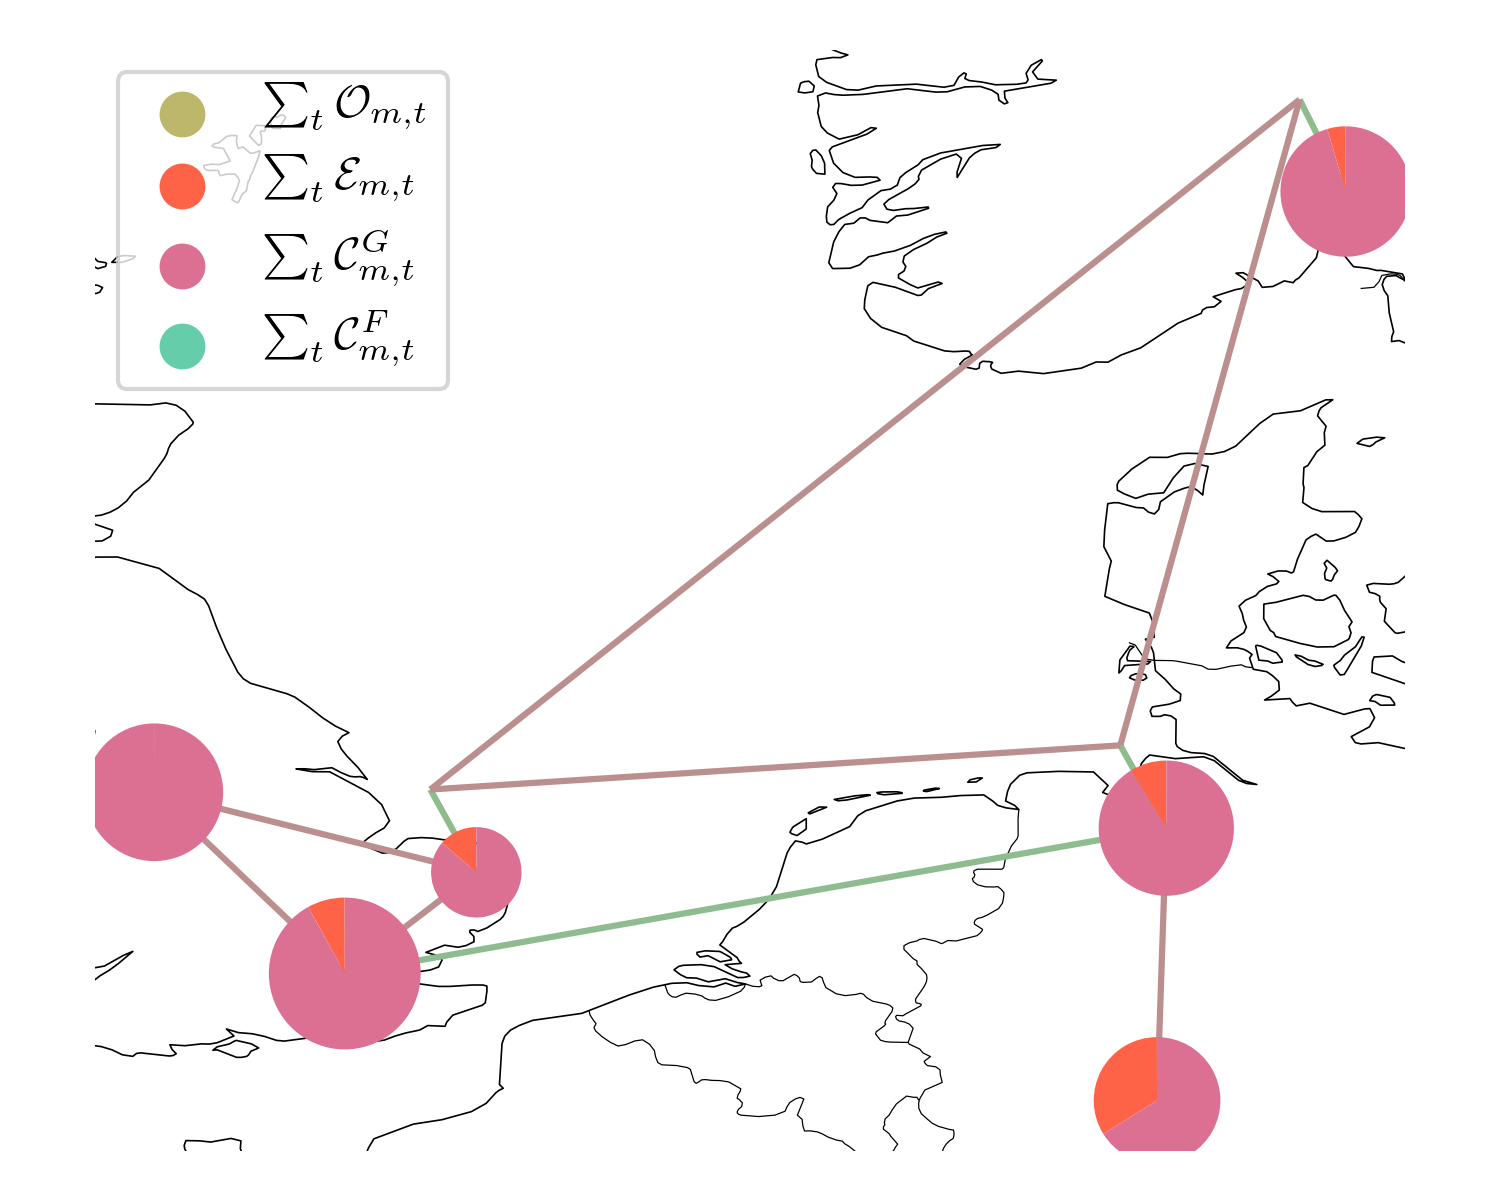
\includegraphics[width=\textwidth]{nodal_payments.png}
    \caption{}
    \label{fig:nodal_payments}
\end{subfigure}
\caption{Network used for showcasing. (a) shows the distributing of generation capacities $\capacityGeneration$, the widths of the transmission lines are proportional to their thermal limit $\capacityFlow$. (b) shows the total nodal payments according to the cost allocation.}
\end{figure}


% 
% 
% 
% \newpage
% \subsubsection*{Relaxed CO$_2$ Constraint}
% 
% 
% \begin{figure}[h]
% \begin{subfigure}{.5\textwidth}
% \centering
%  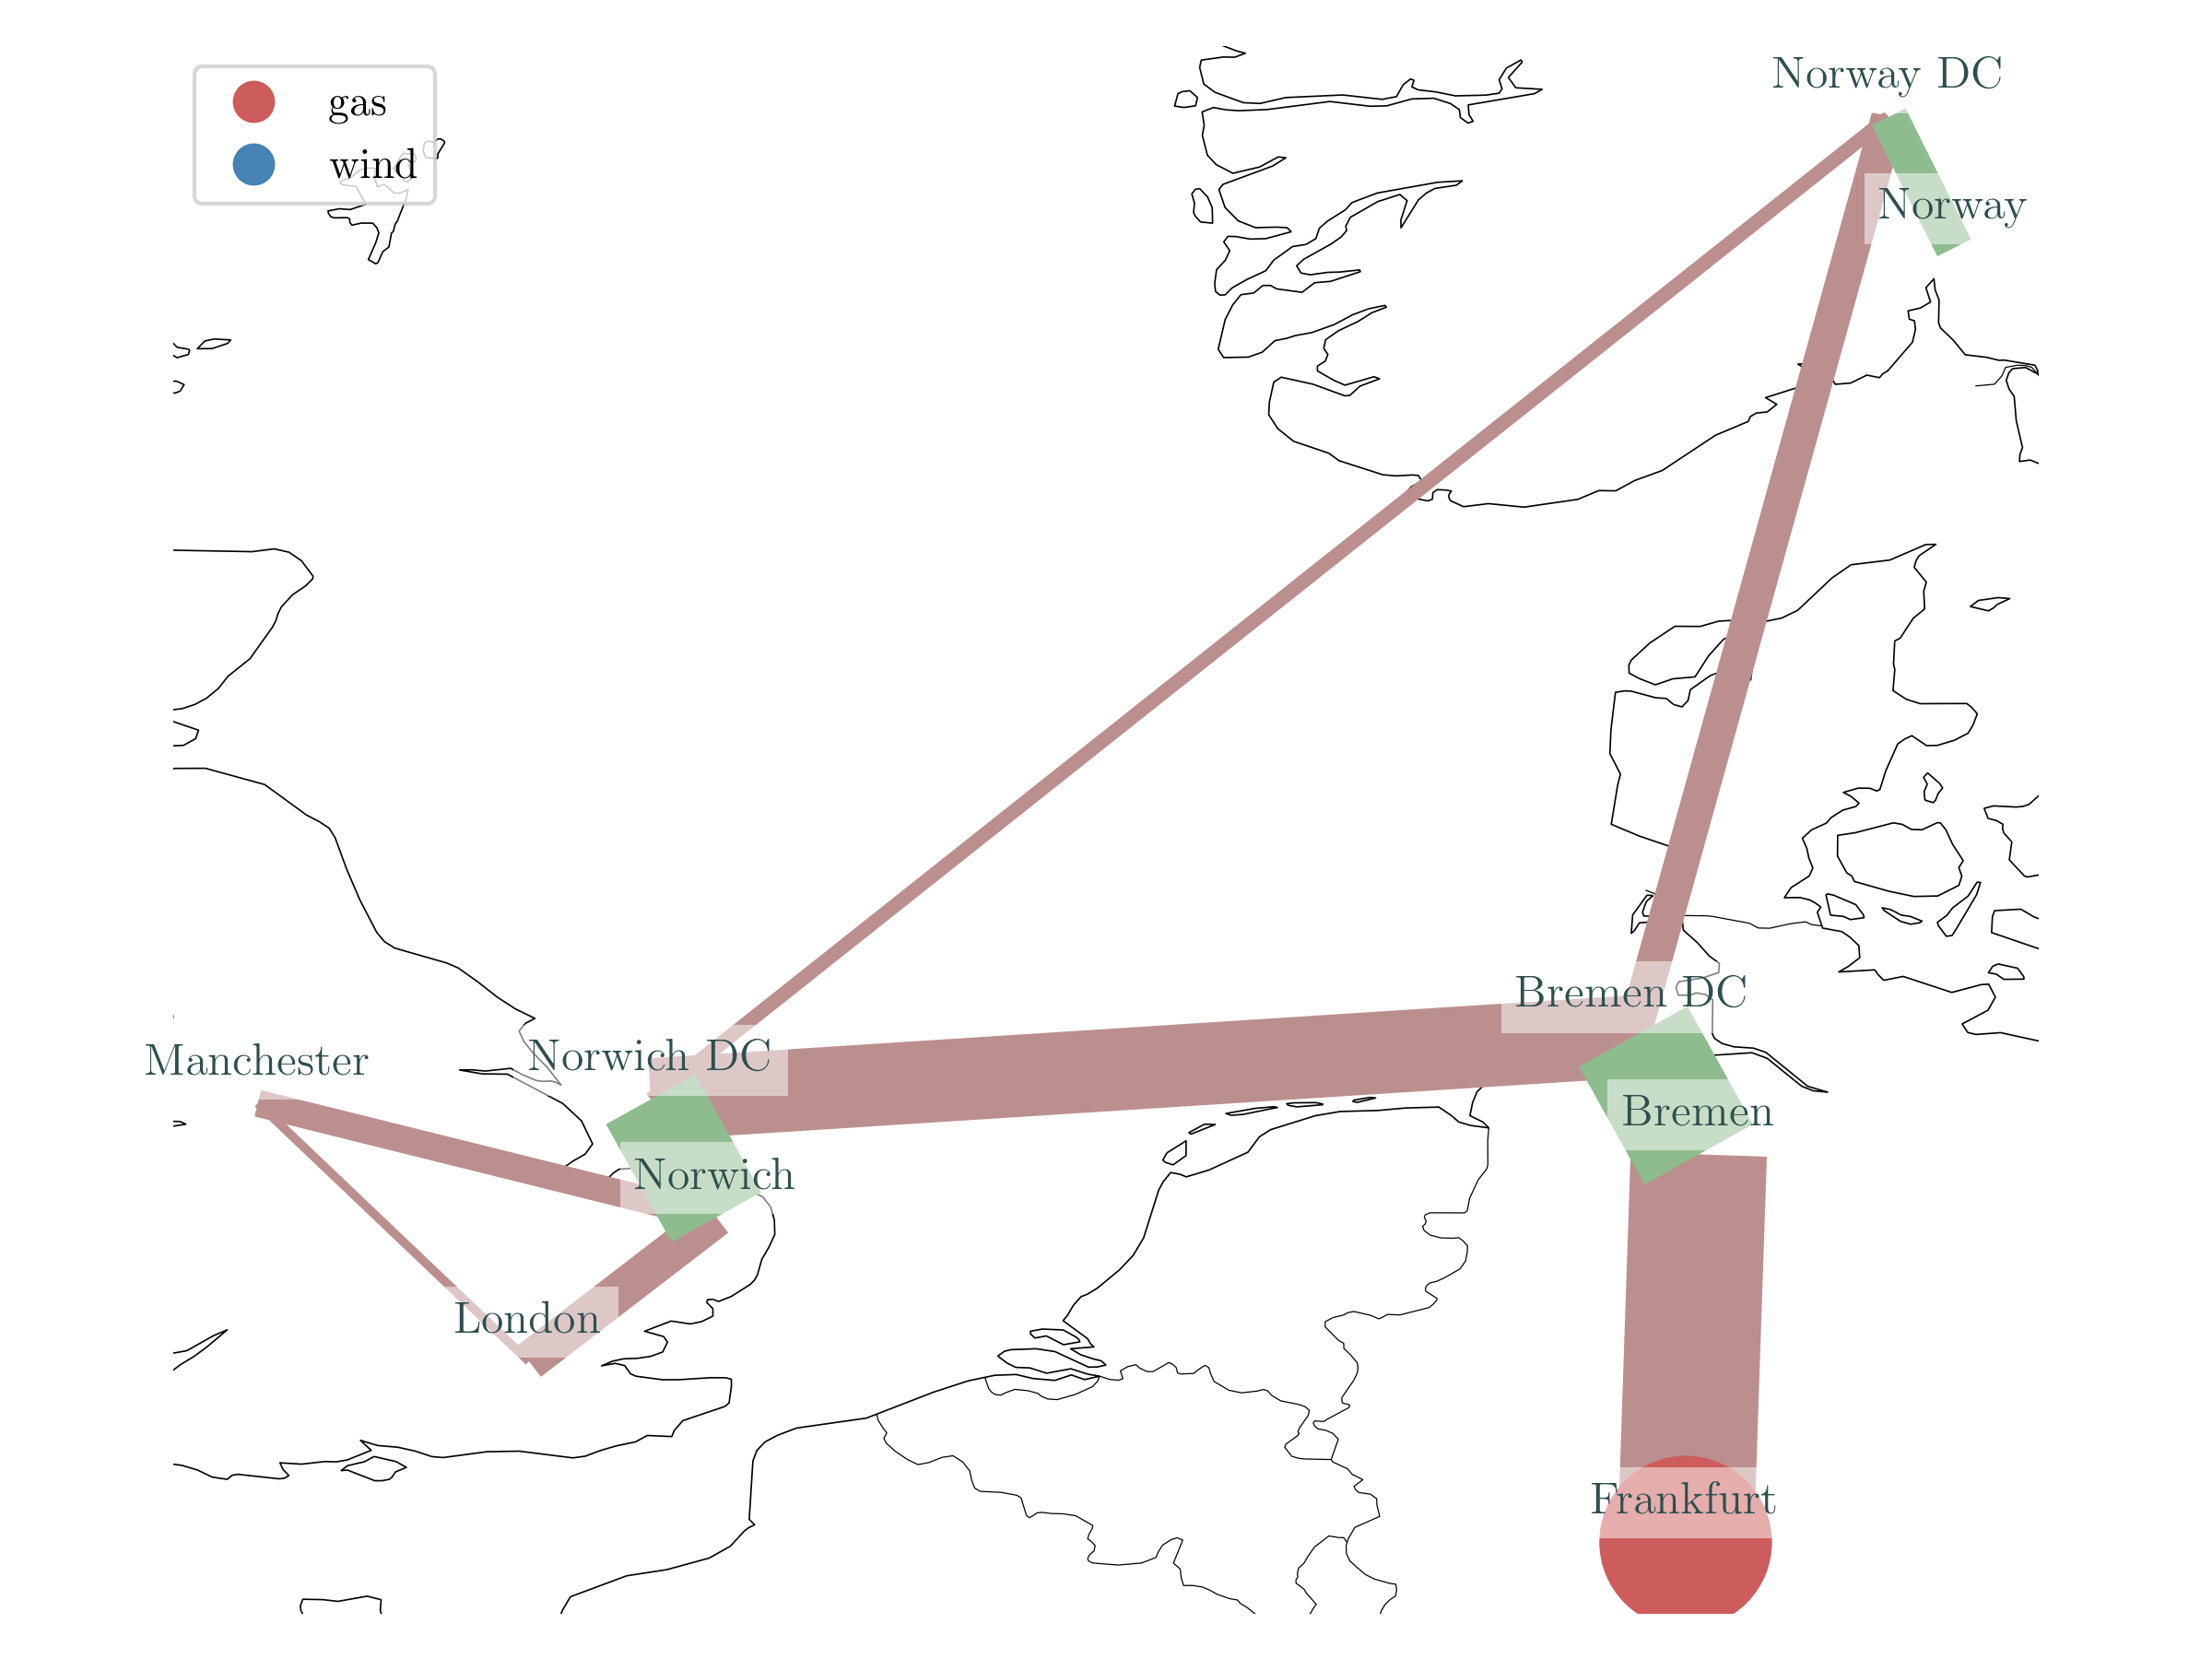
\includegraphics[width=\textwidth]{network_relaxed_co2.png}
%  \caption{}
%  \label{fig:network_relaxed_co2}
% \end{subfigure}
% \begin{subfigure}{.5\textwidth}   
%     \centering
%     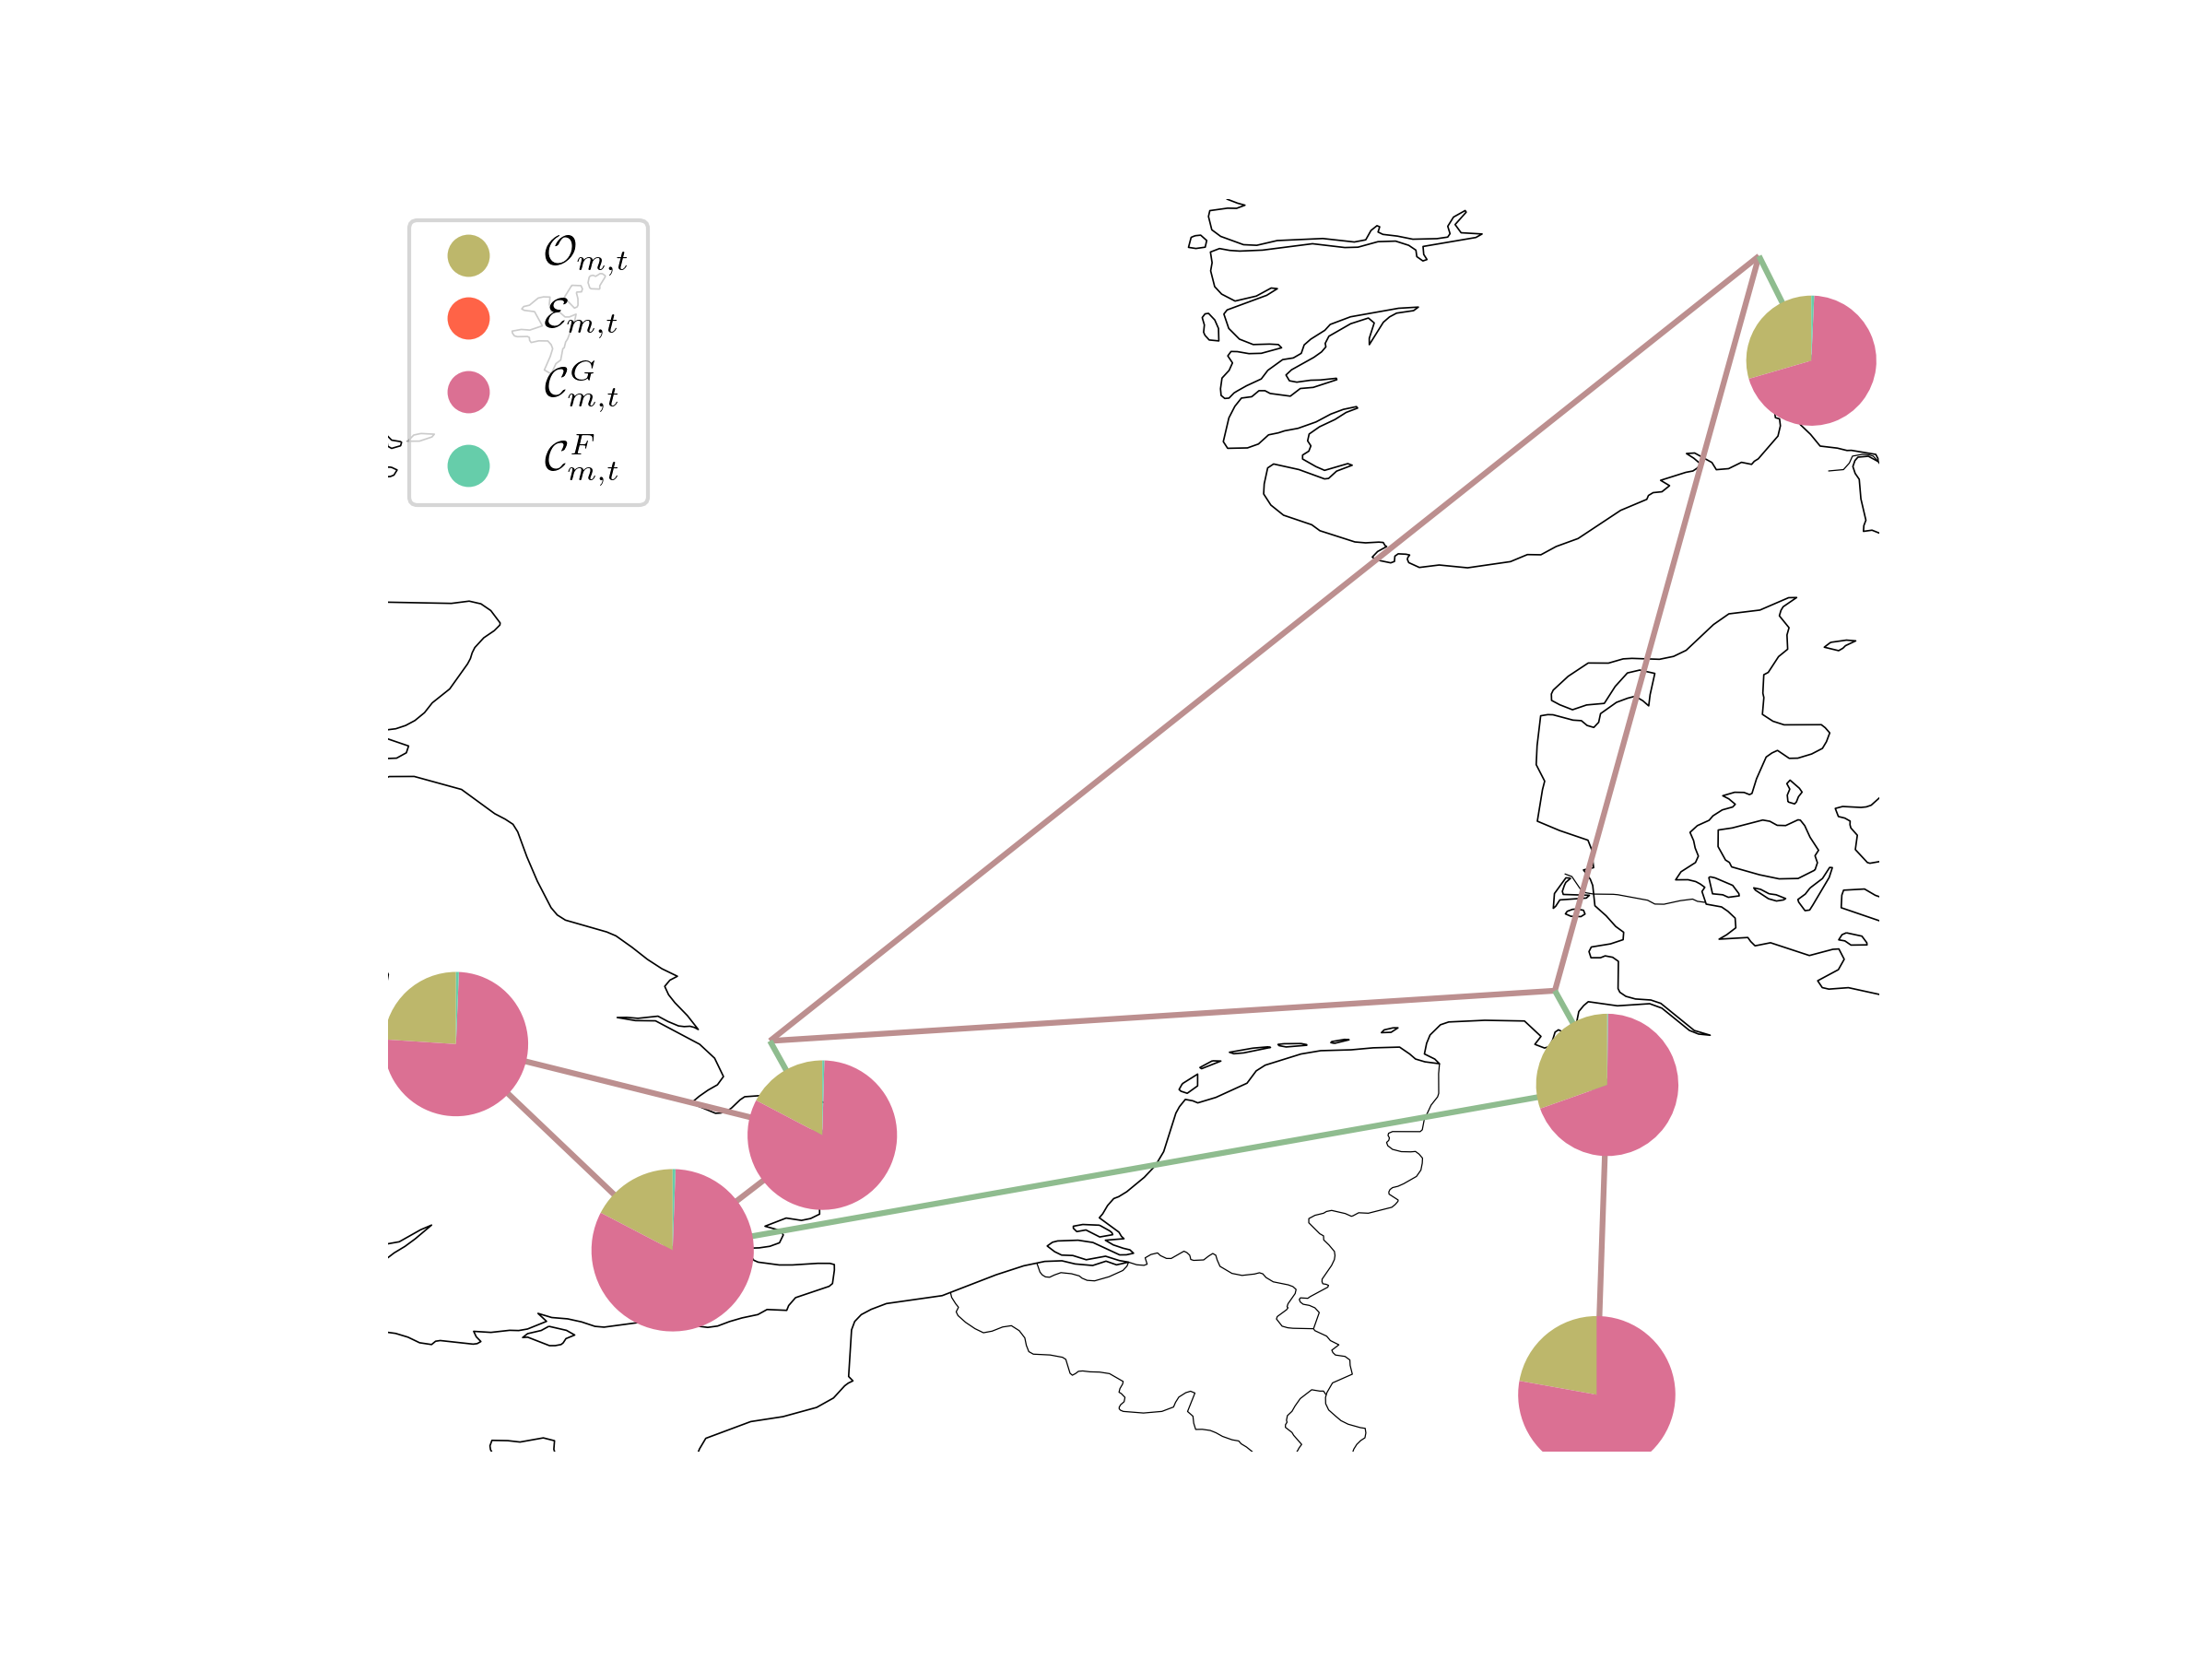
\includegraphics[width=\textwidth]{nodal_payments_relaxed_co2.png}
%     \caption{}
%     \label{fig:nodal_payments_relaxed_co2}
% \end{subfigure}
% \caption{Similar to \cref{fig:network} and \cref{fig:nodal_payments} but without CO$_2$ constraint.}
% \end{figure}
% 
% \begin{figure}[h]
%     \centering
%     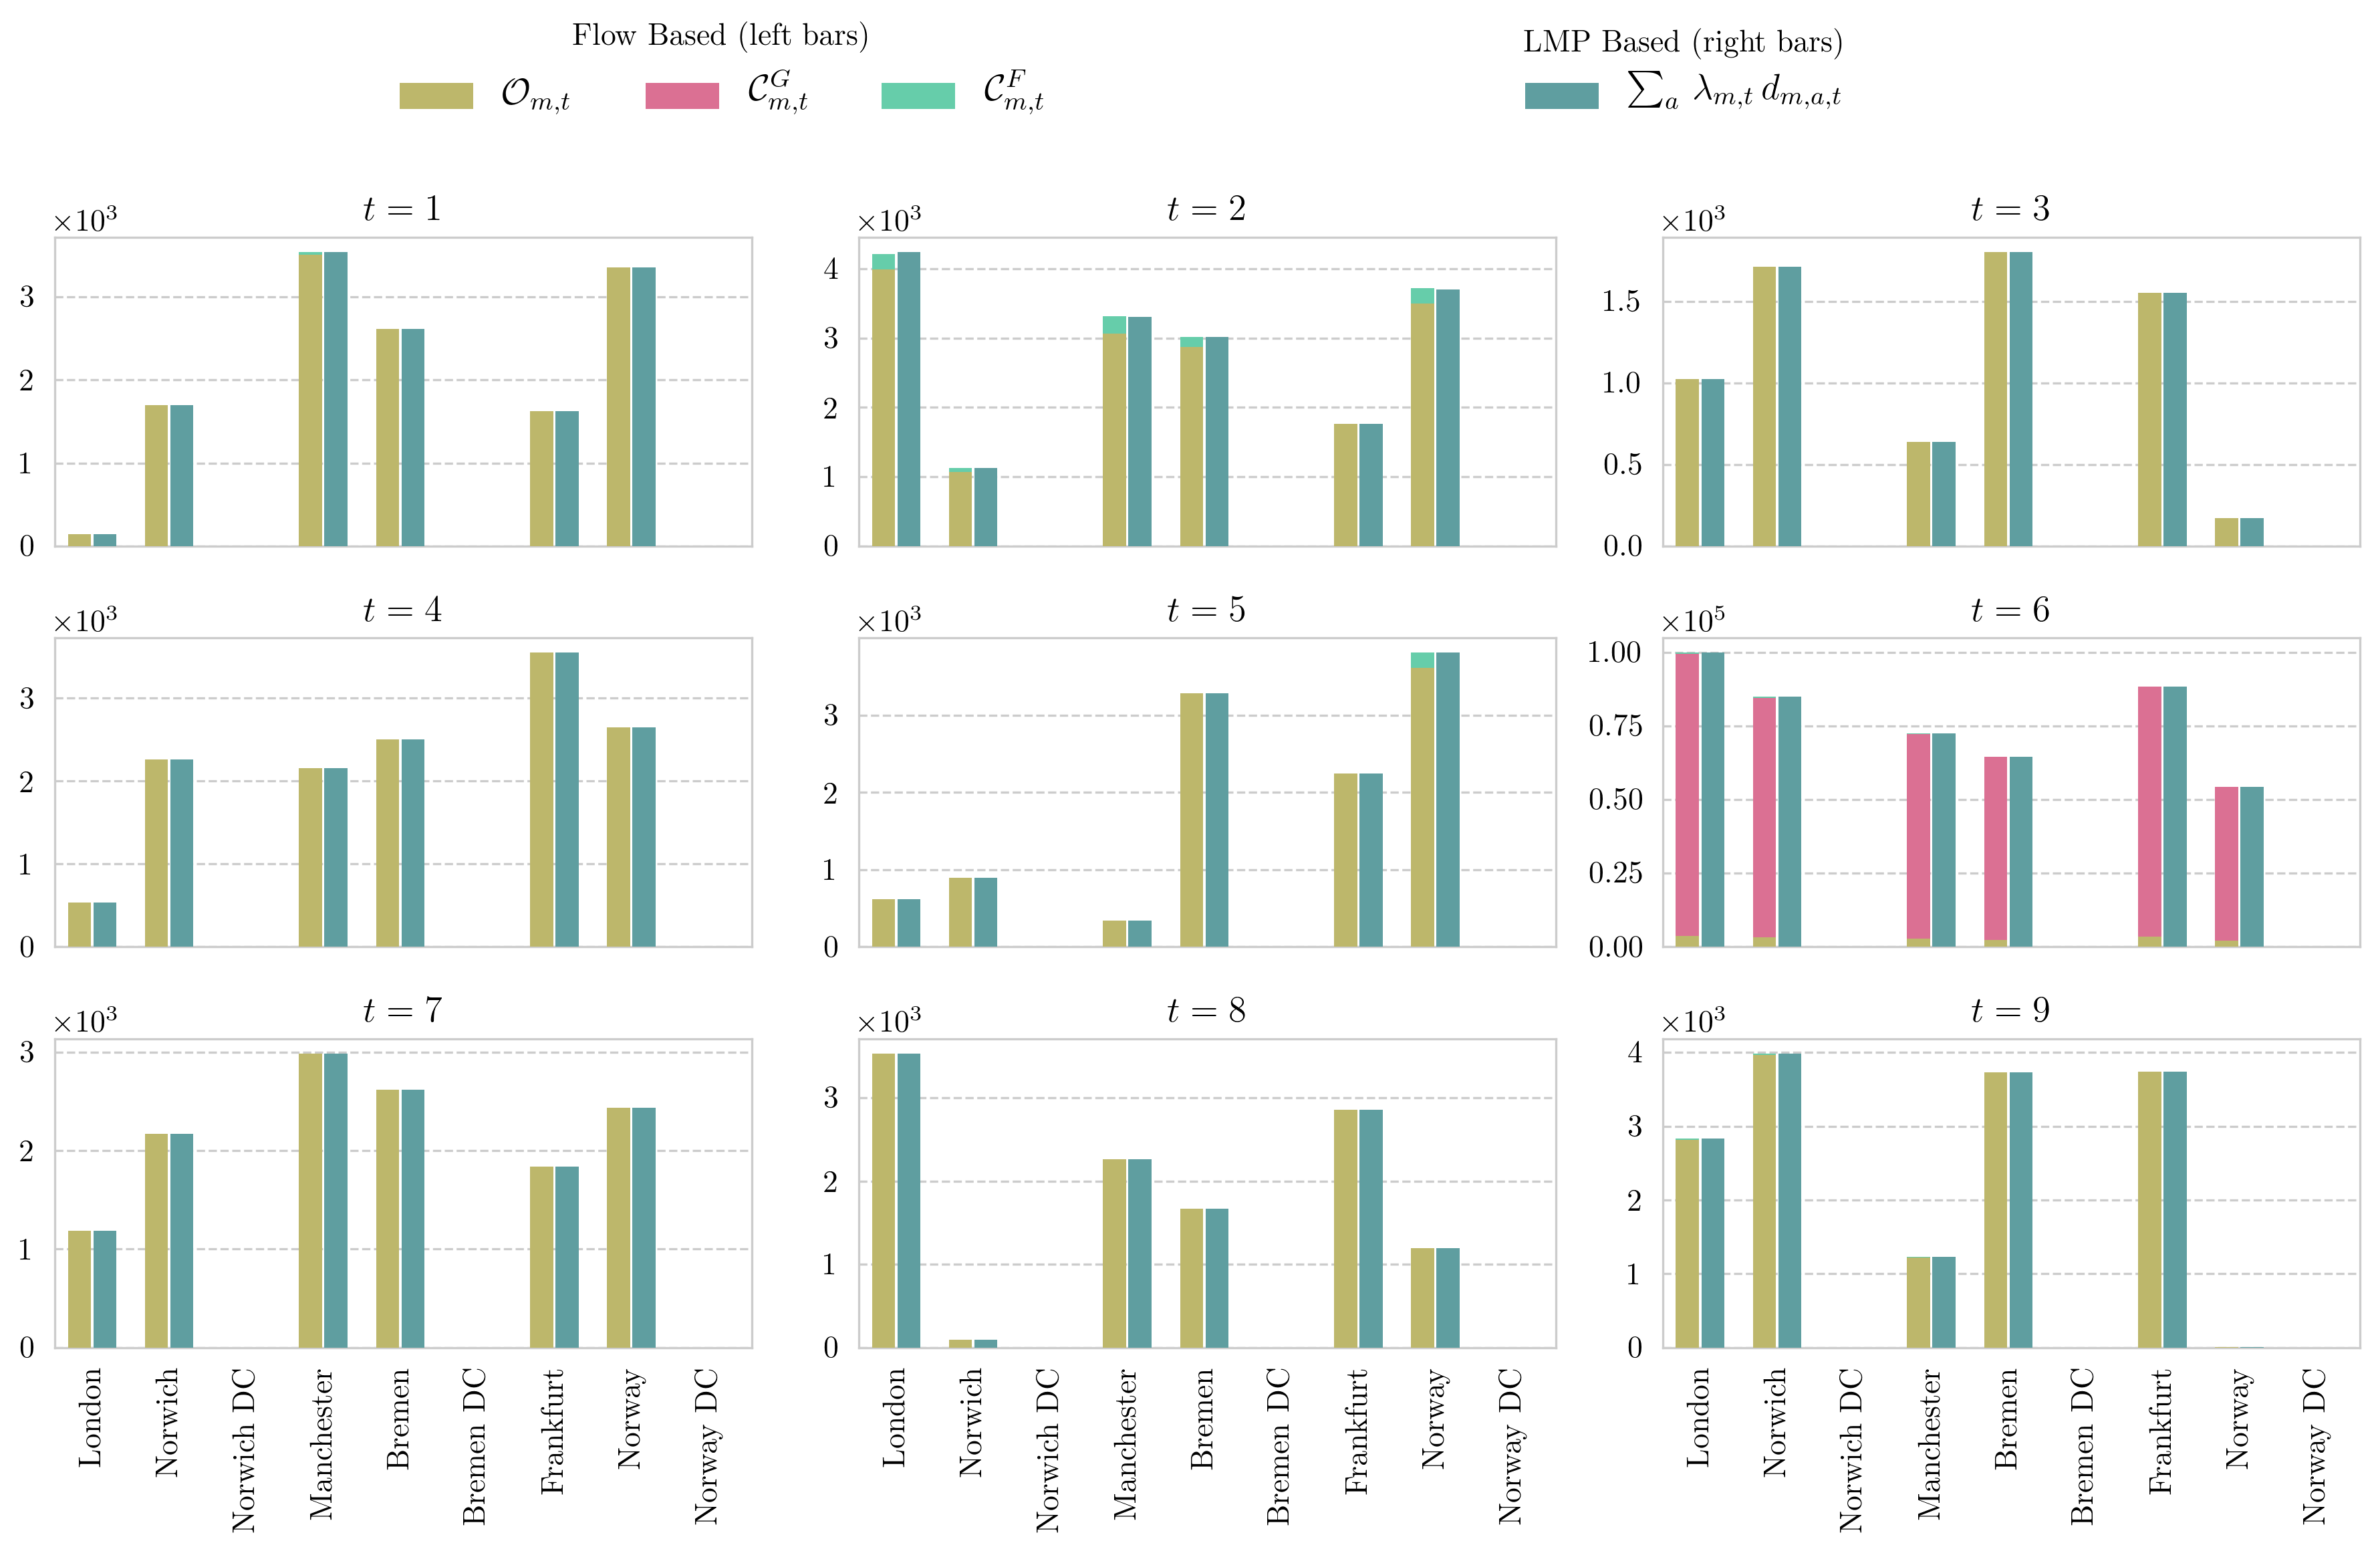
\includegraphics[width=\textwidth]{compare_allocation_relaxed_co2.png}
%     \caption{Comparison of the stacked flow based cost allocation with the LMP based cost per consumer for each time step $t$ without CO$_2$ \cref{eq:co2_constraint}. Only one time-step $t=6$ determines the allocation of generator CAPEX $\allocateCapexGeneration$, as for all other time-steps \cref{eq:upper_generation_capacity_constraint} is not binding. Again note the cost scale difference between time step 6 and all others.}
%     \label{fig:cost_allocation_relaxed_co2}
% \end{figure}
% 
% \subsection*{How does the cost flow through the network}
% 
% \begin{figure}[h]
%     \begin{subfigure}{.5\textwidth}
%       \centering
%       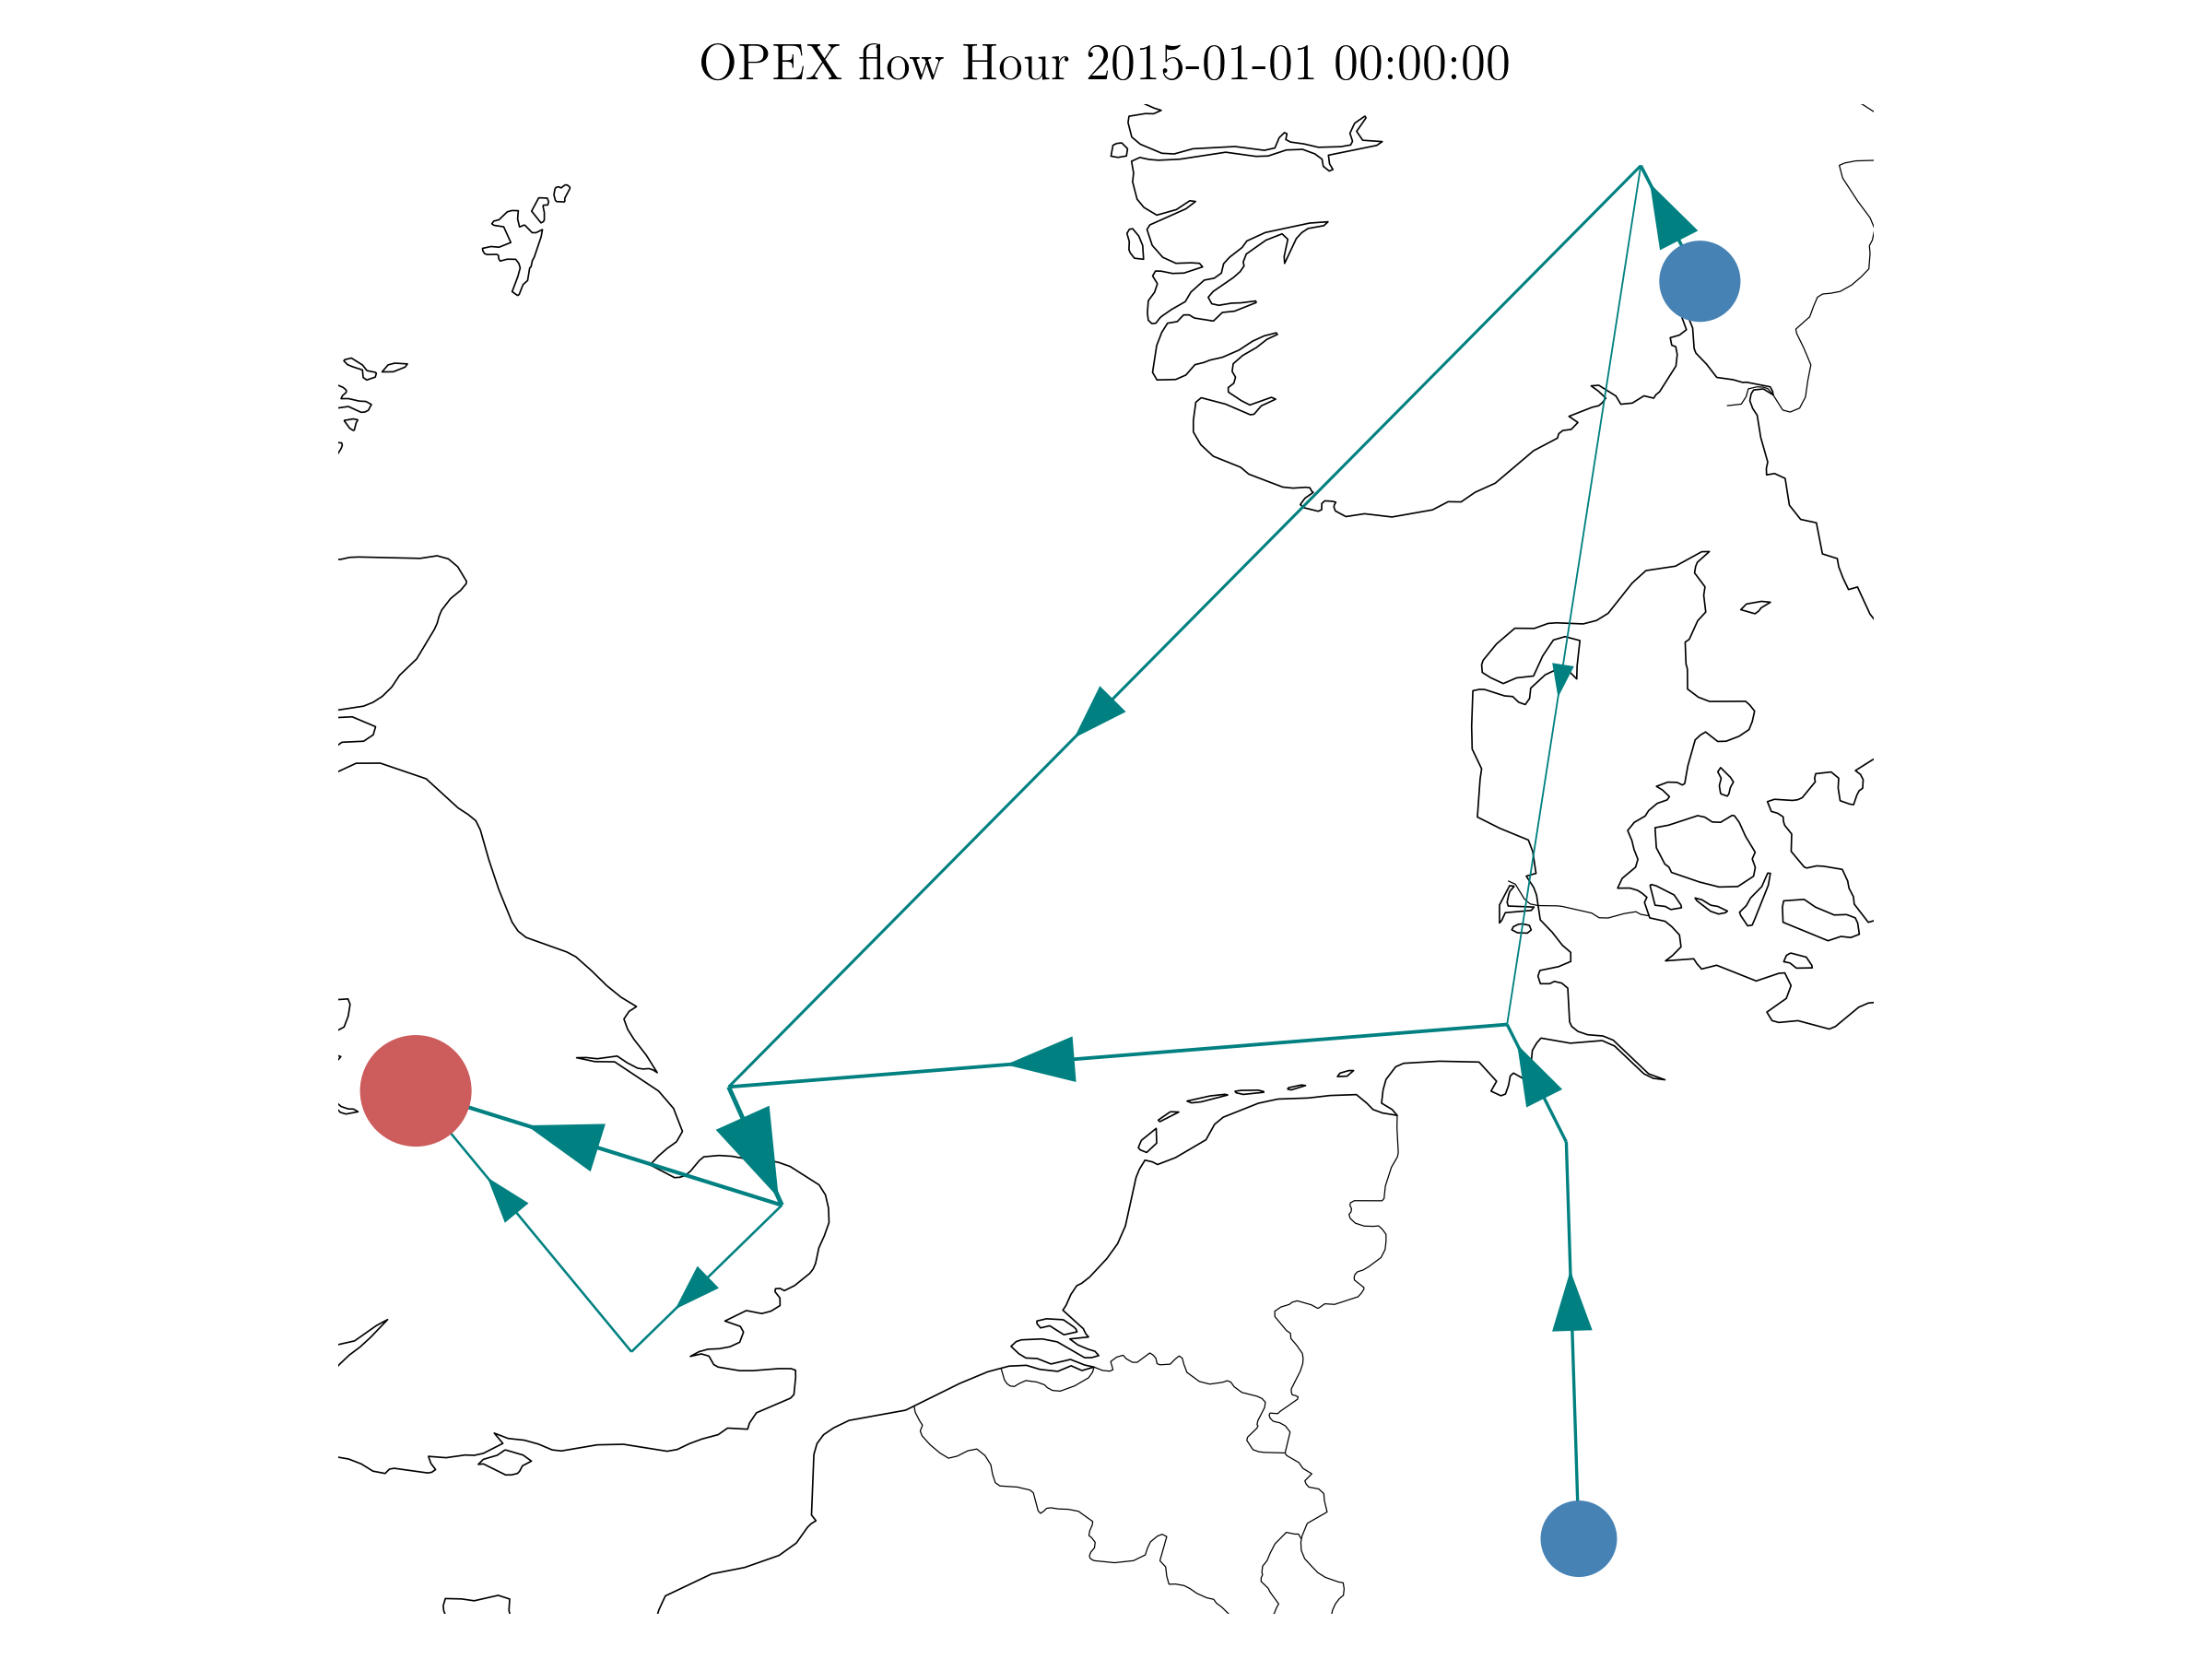
\includegraphics[width=\textwidth]{opex_flow.png}
%       \label{fig:opex_flow}
%     \end{subfigure}%
%     \begin{subfigure}{.5\textwidth}
%       \centering
%       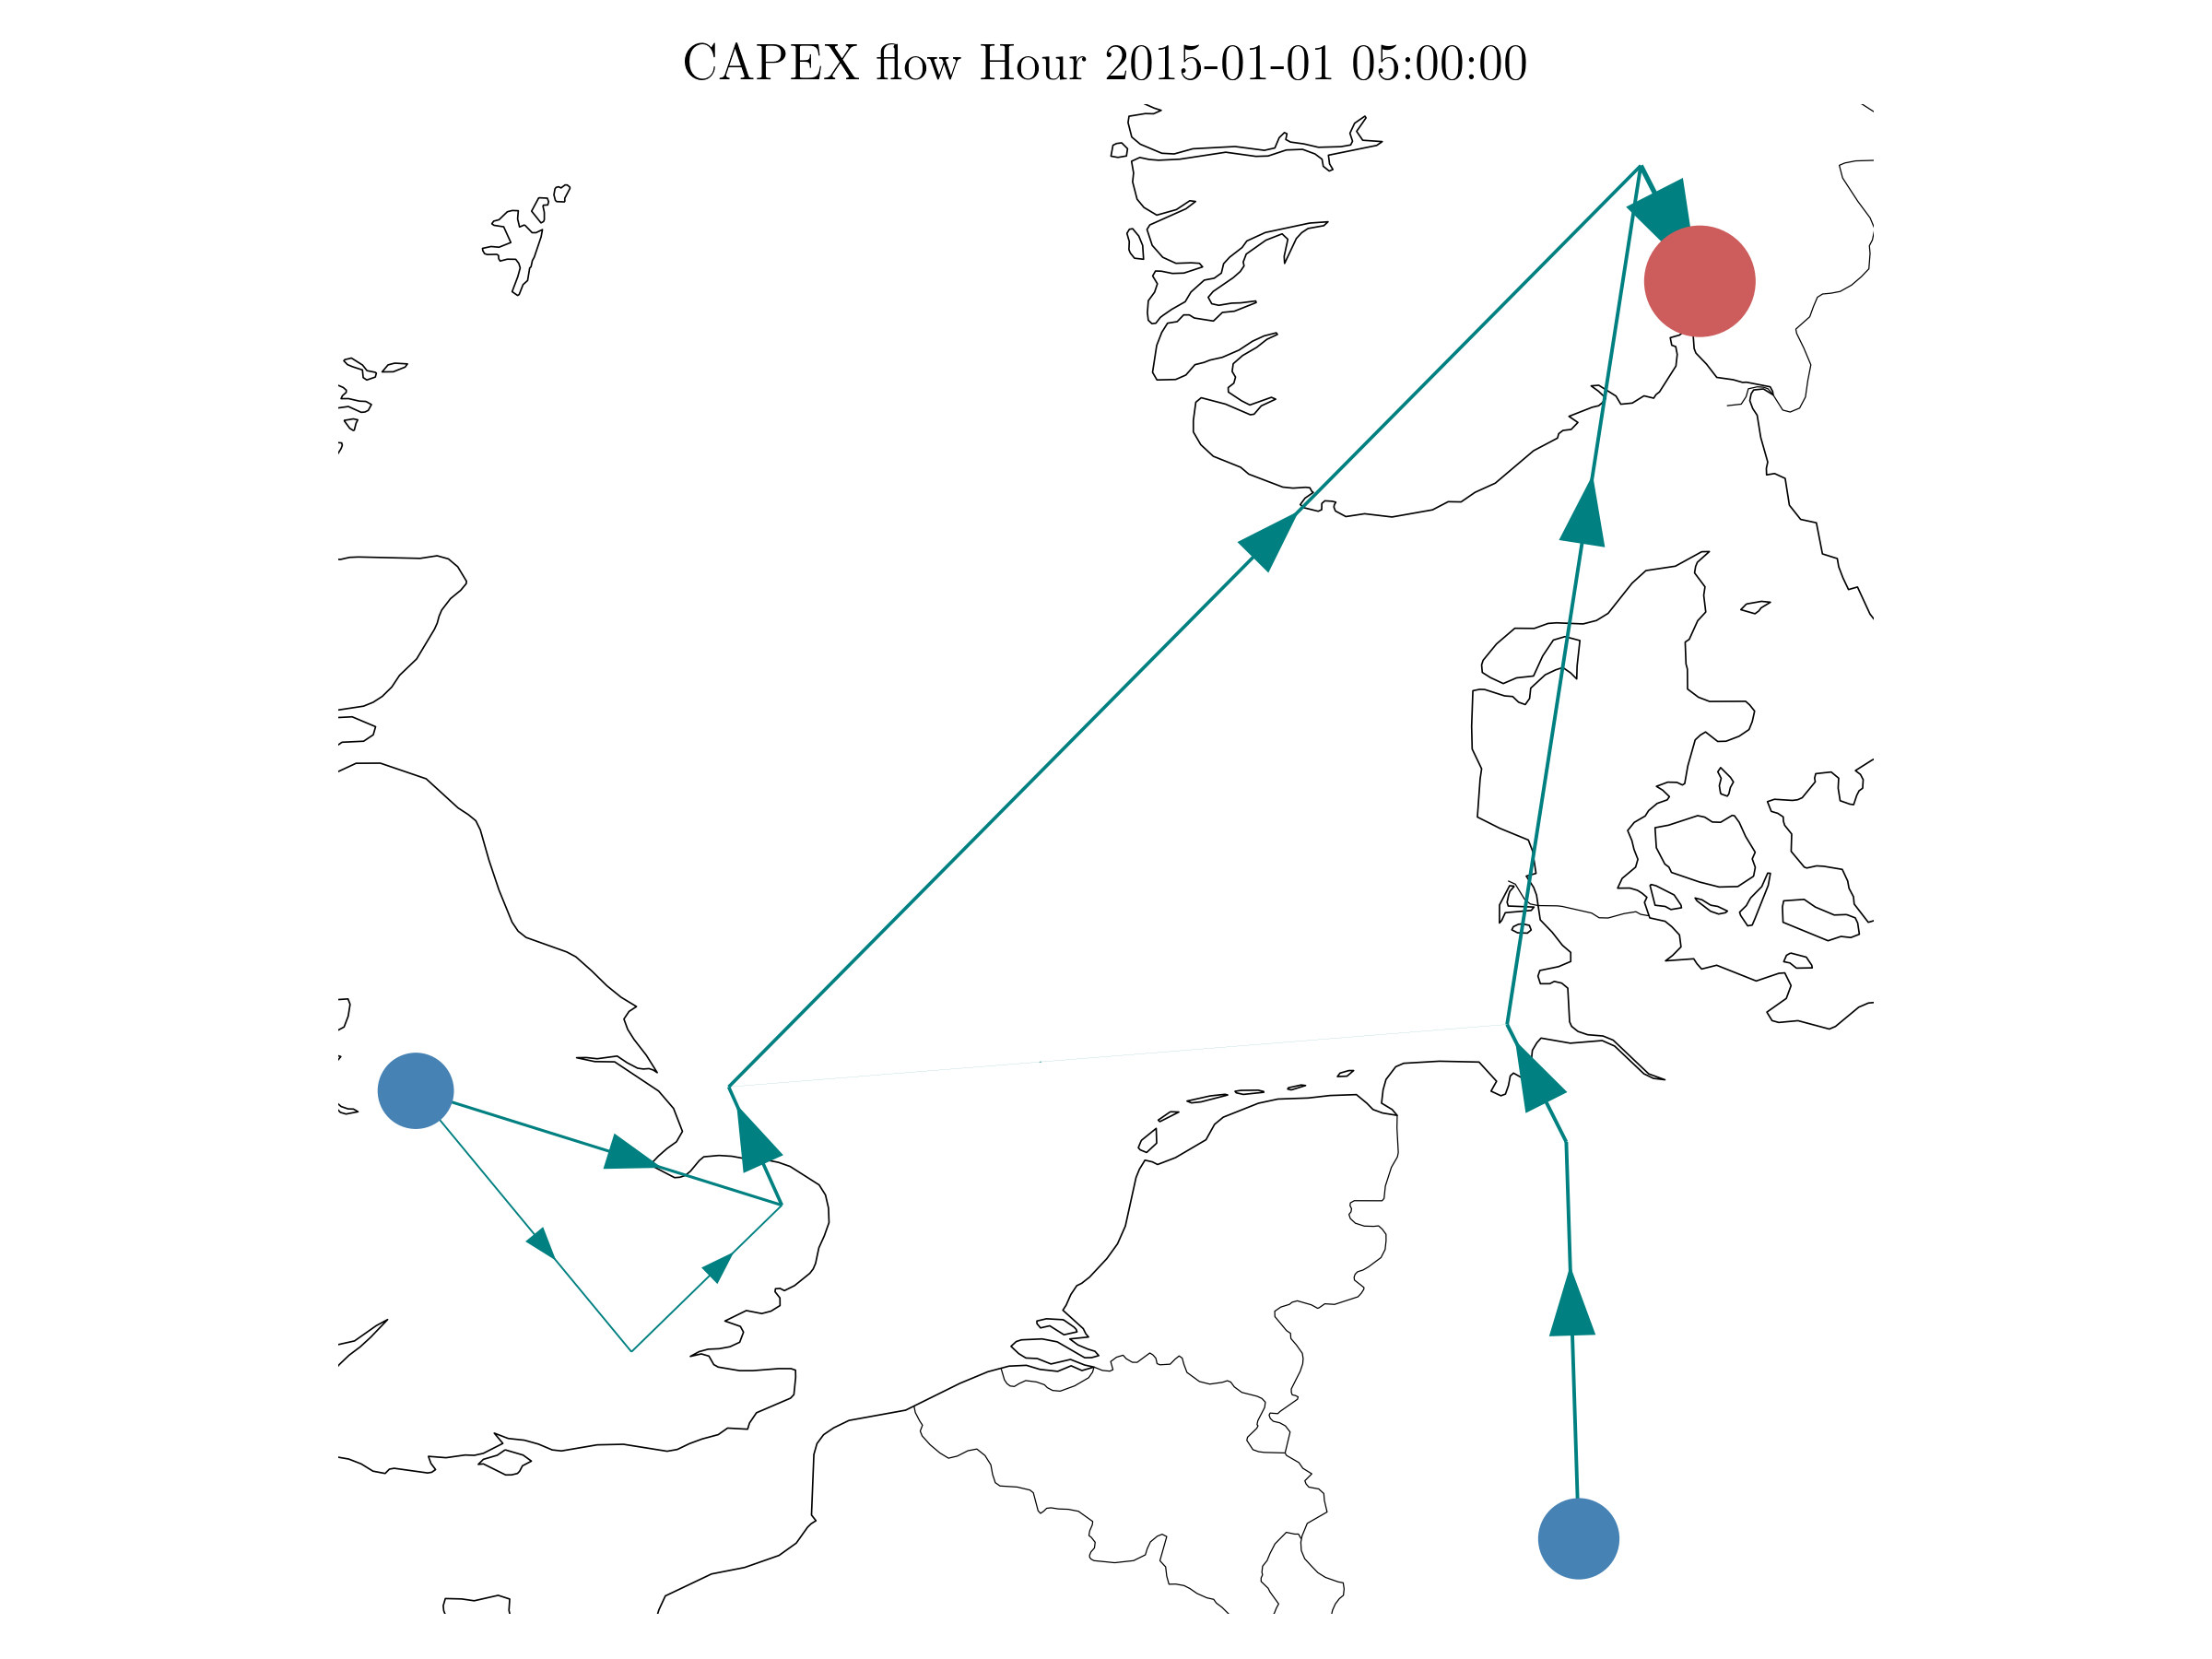
\includegraphics[width=\textwidth]{capex_flow.png}
%       \label{fig:capex_flow}
%     \end{subfigure}
%     \caption{}
%     \label{fig:fig}
% \end{figure}
    
% \begin{appendix}
% Since the P2P comprises all net production and net consumption summing over all sources must result in the nodal demand  
% 
% \begin{align}
%  \sum_{n} \allocatePeer = \sum_a \demand[m]
% \end{align}
% as well as summing over all sinks results in the nodal generation
% \begin{align}
%  \sum_{m} \allocatePeer = \sum_s \generation
% \end{align}
% 
% The P2P relation can be further broke down to allocating generator specific $ \generationshare \, \allocatePeer $ where $\generationshare = \generation/\sum_s \generation$ denotes the share of generator $s$ of the nodel production. Similarly the allocation to consumers a are given by and consumer specific $ \demandshare[m] \allocatePeer$ with the nodal comsumer share given by $\demandshare = \demand/\sum_a \demand$.
% \end{appendix}





% 
% % Direct Coupling:\\
% % \begin{align}
% %  \slack[m] = \dfrac{\generationnodal[m]}{\sum_{n} \generationnodal[n]} 
% % \end{align}
% % 



% \bibliographystyle{ieeetr}
% \printbibliography


\end{document}
